% \documentclass[nofootinbib,english, aip, jcp, priprint, graphicx,floatfix]{revtex4-1}
\documentclass[12pt, nofootinbib,english, amsmath, amssymb, aps, priprint, graphicx,floatfix]{revtex4-1}
\usepackage{amsmath,bm}
\usepackage{amsthm}
\usepackage{amssymb}
\usepackage{mathrsfs}
\usepackage{bbm,latexsym}
\usepackage{graphicx}
\usepackage{cancel}
\usepackage{enumitem}
\usepackage{wrapfig}
\usepackage{setspace}
\usepackage[bottom]{footmisc}

%%%%%%%%%% Start TeXmacs macros
\newcommand{\mathd}{\mathrm{d}}
\newcommand{\nin}{\not\in}
\newcommand{\tmop}[1]{\ensuremath{\operatorname{#1}}}

\newcommand{\theepsrate}{\varepsilon + \sqrt{\varepsilon/2}}
\newcommand{\tmtextbf}[1]{{\bfseries{#1}}}
\newtheorem{definition}{Definition}
\newtheorem{proposition}{Proposition}
\newtheorem*{proposition*}{Proposition}
\newtheorem*{corollary*}{Corollary}
\newtheorem*{corollary}{Corollary}
\newtheorem{theorem}{Theorem}
\newtheorem{lemma}{Lemma}
\newtheorem{algorithm}{Algorithm}
%%%%%%%%%% End TeXmacs macros

% \draft % marks overfull lines with a black rule on the right

\theoremstyle{plain}
\newtheorem{thm}{\protect\theoremname}
\newtheorem*{thm*}{\protect\theoremname}
\newtheorem*{lem*}{\protect\lemmaname}
\theoremstyle{definition}
\newtheorem{defn}[thm]{\protect\definitionname}
\theoremstyle{plain}
\newtheorem{cor}[thm]{\protect\corollaryname}

\newcommand{\normal}{{\mathfrak{n}}}
\newcommand{\TODOTHIS}{{\huge !!!!}}
\newcommand{\indicatorf}[1]{\mathbb{I}_{#1}}
\newcommand{\capac}[2]{\ensuremath{\operatorname{cap}}(#1,#2)}
\newcommand{\hatcapac}[2]{\ensuremath{\operatorname{\widehat{cap}}}(#1,#2)}
\newcommand{\hausdorffmeasure}{\mathscr{H}(dx)}
\newcommand{\PMeasure}{\mathscr{P}(dx)}
\newcommand{\tPMeasure}{\tilde{\mathscr P}(dx)}
\newcommand{\fnsp}{\mathscr{H}^1}
\newcommand{\bb}[1]{\mathcal{B}\left(#1\right)}
\newcommand{\BB}[1]{\mathcal{\bar B}\left(#1\right)}


\usepackage[english]{babel}
\providecommand{\corollaryname}{Corollary}
\providecommand{\propositionname}{Proposition}
\providecommand{\definitionname}{Definition}
\providecommand{\lemmaname}{Lemma}
\providecommand{\theoremname}{Theorem}

\newcommand{\dA}{{\dot A}}
\newcommand{\tA}{{\tilde A}}
\newcommand{\dB}{{\dot B}}
\newcommand{\tB}{{\tilde B}}
\newcommand{\capA}{\kappa_A}
\newcommand{\capB}{\kappa_B}

\parskip=1pt
\usepackage[compact]{titlesec}
\titlespacing{\section}{0pt}{20pt}{20pt}
\titlespacing{\subsection}{0pt}{*0}{*0}
\titlespacing{\subsubsection}{0pt}{*0}{*0}

\begin{document}

\title{Capacities and the Efficient Computation of First 
Passage Probabilities} %Title of paper

\author{Jackson Loper}
\thanks{These two authors contributed equally}
\affiliation{Data Science Institute, Columbia University, New York, NY, USA}

\author{Guangyao Zhou}
\thanks{These two authors contributed equally}

\author{Stuart Geman}
\thanks{Partially supported by the Office of Naval Research under contracts ONR N000141613168 and ONR N000141512267}
\affiliation{Division of Applied Mathematics, Brown University, Providence, RI, USA}
\date{\today}

\begin{abstract}
	A reversible diffusion process is initialized at position $x_0$ and run until it first hits any of several targets.  What is the probability that it terminates at a particular target? We propose a new approach for estimating this probability, focused on those situations in which it takes a long time to hit any target. In these 
cases,  direct simulation of the hitting probabilities becomes prohibitively expensive.  On the other hand, if the timescales are sufficiently long then the system will essentially ``forget'' its initial condition before it encounters a target.  In these cases the hitting probabilities can be accurately approximated using only local simulations around each target, obviating the need for
direct simulations.  In empirical tests, we find that these local estimates can be computed in the same time it would take to compute a single direct simulation, but that they achieve an accuracy that would require thousands of direct simulation runs.
\end{abstract}

\pacs{}% insert suggested PACS numbers in braces on next line

\maketitle %\maketitle must follow title, authors, abstract and \pacs

\section{Introduction}
\label{sec:Introduction}

Reversible diffusions play a key role in a wide variety of physical systems.  For example, the folding of macromolecules into their native configurations is often posed as a diffusion (either directly through simulations of atomic dynamics or indirectly through mesoscopic models \cite{Scheraga2007-qw,Hospital2015-ol,lei2010direct}), the fluctuation of chemical species in solution can be modeled as diffusions (``chemical Langevin equations'' are one classic example of this approach \cite{sotiropoulos2011analytical,gillespie2000chemical}), the motion of particles through membranes can be posed as a diffusion \cite{holcman2004escape}, and so-on.   In all cases, the the physical state of the system at time $t$ is represented through a variable $X_t$, confined to a finite region $\Omega$ and evolving according to a stochastic differential equation.  

In this paper we seek to estimate first-passage probabilities 
(sometimes also called ``splitting probabilities'' \cite{E2006-fm} or simply ``hitting probabilities'')
of such diffusions: given an initial condition $x_0$ and a collection of targets, what is the probability that the process first hits any particular target before hitting any of the other targets? Targets might represent, for example, multiple  exit locations from a region of the state space in a statistical mechanics problem or the establishment of new intra-molecular bonds in a folding problem. Where will the system first exit or  what is the next step in folding?  This paper develops a new algorithm for the  approximation of first-passage probabilities.

To keep things simple, most of the discussion will be in the context of just two targets, $A$ and $B$, $A,B\subset\Omega$, although all of the results apply, with trivial notational changes, to any finite set of targets. In this context, ``hitting probability'' 
(aka  ``first-passage probability'') refers to the specific probability that $X_t$ hits target $A$ before target $B$.  
The algorithm is designed for cases where the diffusion ``forgets'' its initial condition before encountering a target.  Precise definitions are in \S\ref{sec:Preliminaries}, but to get the main idea consider a region $M$ in $\Omega$ that lies outside of the targets $A$ and $B$, $M\subset \Omega\backslash(A\cup B)$,
and assume that the diffusion starts in $M$ ($x_0\in M$).
Recall that reversible diffusions are {\em ergodic}: as time goes on, it gets harder and harder to guess the initial condition from the current configuration.  As this happens, the process is said to become ``mixed,'' and the speed with which the initial condition is forgotten is called the ``mixing rate.''  If the first passage time out of $M$ is long relative to this mixing rate, then the hitting probability will be nearly independent of $x_0$. This is what we mean by ``forgets'' its initial condition. Our main result (Theorem \ref{thm:main_thm}) asserts that if the
hitting probability varies by at most $\varepsilon$ among all initial conditions in $M$, then the proposed algorithm's approximation error is less than $\varepsilon + \sqrt{\varepsilon/2}$.  Figure \ref{fig:ToyModel} gives a rough sketch of this idea.  

When would these conditions hold? We will have more to say about this in \S\ref{sec:MainResults}, but for now we note that the narrow-escape literature gives at least one class of examples.  In these examples $X_t$ is a Brownian motion trapped inside a set by reflecting boundaries, and the targets are very small windows in boundary.  These models have been successfully applied to a variety of mesoscopic biosystems (cf. \cite{schuss2007narrow} and the references therein).  These kinds of diffusions may also be relevant for modeling the folding of large molecules.  According to McLeish,  ``folding rates are controlled by the rate of diffusion of pieces of the open coil in their search for favorable contacts'' \cite{McLeish2005-dq}.  There is also some experimental evidence that the exploration of large regions is the rate-limiting step for a variety of processes \cite{Goldberg1999-mv,Jacob1999-bs,Plaxco1998-iv,Wales2006-ur}.  If these results bear out, then to the extent that exit times are long it will be possible to obtain good approximations for hitting probabilities using our approach.

Many standard methods for calculating hitting probabilities fail for diffusions of this kind.  When the escape time from $M$ is large, the associated partial differential equations often include large Lipschitz constants and direct Monte-Carlo simulation requires a prohibitive number of timesteps (cf.\ \cite{Baum1986-we, Wille1987-tf, Machta2009-gh}).  Some authors take a pessimistic view on this subject: ``If these processes are intrinsically slow, i.e. require an extensive sampling of state space, not much can be done to speed up their simulation without destroying the dynamics of the system'' \cite{Christen2008-ge}.
But in fact diffusions of this kind enjoy certain properties which can actually make analyses easier.  The literature includes a variety of tools which use such properties to advantage.  Here we review a few of these tools:

\begin{description}
    \item[Analytic analyses] When targets are very small, the first-passage {\em times} (as opposed to probabilities) are often well-approximated by analytic formulas.  The narrow-escape literature has developed many techniques in this direction.  Much of this literature focuses on making these formulas as accurate as possible for specific geometric configurations, such as the case of $N$ circular targets (cf.\ \cite{cheviakov2010asymptotic}), the case that one target lies at the end of a long tube (cf.\ \cite{li2014matched}), or the case that the motion is trapped inside a symmetric domain (cf.\ \cite{Chevalier2010-bq,Condamin2006-vi,Coombs2009-pe,Lindsay2017-ds}).  There is also some work on efficient numerical methods for low-dimensional problems using insights from these analytic results (cf.\ \cite{kaye2019fast}).  Note that this literature mostly focuses on hitting times, whereas in this paper we focus on hitting probabilities.  
Nevertheless, the first-passage probabilities are nearly inversely proportional to the mean first-passage times for many cases, so these techniques can often be used to estimate first-passage probabilities.  A helpful overview of many of the main ideas in this literature can be found in \cite{Benichou2014-jb}.

    \item[Markov State Models] Markov State Models (MSM) begin by partitioning the state-space of the diffusion into $n$ sets (``states'').  The diffusion can be understood at a coarse level by looking at which state the process is in at any given time (cf.\ \cite{Pande2010-yi, Chodera2014-bh, Husic2018-xp}).   In some cases the time it takes to move between states is long relative to the rate of mixing inside the states.  This separation of timescales ensures that the coarse process is approximately Markovian.  We can therefore approximately simulate the discrete process as long as we know the distribution on the exit times and the probability of transitioning to each possible state.  The amount of computational time required to simulate from this approximate process does not depend upon how long the process actually spends in each state.

    \item[Site-localizing functions] Site-localizing functions define a kind of continuous version of the MSMs: instead of creating a hard partitioning of the space, one constructs basis functions $g_1(x)\cdots g_n(x)$ such that $\sum_i g_i(x)=1$.  In many cases the action of the relevant diffusion operators can be well-approximated by the their action on the $n$-dimensional space spanned by these basis functions.   For example, under a separation-of-timescales assumption, Morro (cf.\ \cite{moro1995kinetic}) shows a way to design basis functions which faithfully represent the diffusion's behavior on the slow timescale.

    \item[Milestoning] In some cases it is possible to construct a low-dimensional reaction coordinate which measures the distance from the targets in some suitable metric.  In some cases the movement along this reaction coordinate is slow relative to the mixing rate along all other directions.  This separation of timescales ensures that the dynamics of the diffusion along this coordinate are approximately Markovian.  If the reaction coordinate is carefully chosen, many properties of the original diffusion are maintained in this low-dimensional projection \cite{E2006-fm}.  Simulating the low-dimensional approximate diffusion can yield useful insights into the behavior of the original system \cite{Bello-Rivas2015-ld}.  
\end{description}

Here we will investigate a different way to make use of separated timescales. Let $h_{A,B}(x)$ denote
the probability of hitting $A$ before $B$ given that the diffusion
is initialized at $x\in M$.
It is well known that $h_{A,B}(x)$ can be represented as the 
solution of a variational problem. (A detailed account of this and related facts is included in Appendix \ref{sec:three_perspectives}.)  Under the special condition that $h_{A,B}(x)$ is a constant, say 
$h_{A,B}(x)=\bar{h}$ for all $x\in M$, the solution of the variational problem, and hence $\bar{h}$, can be written in terms of certain integrals over local regions surrounding the targets
(indicated by
the gray-shaded areas in the examples depicted in Figure \ref{fig:ToyModel}).
We will refer to these integrals as 
``first-passage capacities''---see \S\ref{sec:Preliminaries} for the
formal definition. If, on the other hand, $h_{A,B}(x)$ is not exactly constant, then $\bar{h}$ becomes an approximation rather than an exact formula: for all $x\in M$,
$|\bar h - h(x) |\leq \varepsilon + \sqrt{\varepsilon/2}$, where $\varepsilon$ is the difference between the maximum and minimum hitting probabilities over $M$. This is the main theoretical result---Theorem \S\ref{thm:main_thm}---which reduces the first-passage problem to one of evaluating local integrals. 
For the purpose of evaluating these integrals, we introduce a Monte Carlo approach, that we call the shell method, and  demonstrate its accuracy and computational efficiency.

The key advantage of our approach is that it allows us to get good estimates while completely ignoring all dynamics inside $M$.  This is particularly valuable if $M$ is a large, high-dimensional set.  In this case it is unclear how one would partition $M$ or formulate a meaningful reaction coordinate, calling into question the utility of Markov State Models and milestoning under these conditions.  Furthermore, integrating over all of $M$ is computationally burdensome, making site-localizing functions also difficult to implement.  Asymptotic techniques from the narrow escape/reaction-controlled diffusion literature may still be applied, but only if the problem falls into one of a collection of very specific cases, most of which lie in two or three-dimensions, feature regular targets, and assume that the diffusion has no energetic potential.  By contrast, 
first-passage capacities can be calculated efficiently for a diffusion with an arbitrary energetic potential, target shape, and ambient dimension.  Moreover, first-passage capacities are fundamentally non-asymptotic quantities; for any problem the approximation error is bounded explicitly in terms of the extent to which the hitting probability varies across $M$.  On the other hand,
the strengths of the capacity-based approach are accompanied by a significant limitation: the approach gives no information about first-passage {\em times}. Indeed, the temporal process is explicitly eliminated. In general, there is an overall proportionality constant which connects first-passage hitting probabilities to first-passage hitting times, but this relationship cannot be recovered from the first-passage capacities.  We discuss this limitation further in \S\ref{sec:Discussion}.
 

\begin{figure}
    \centering  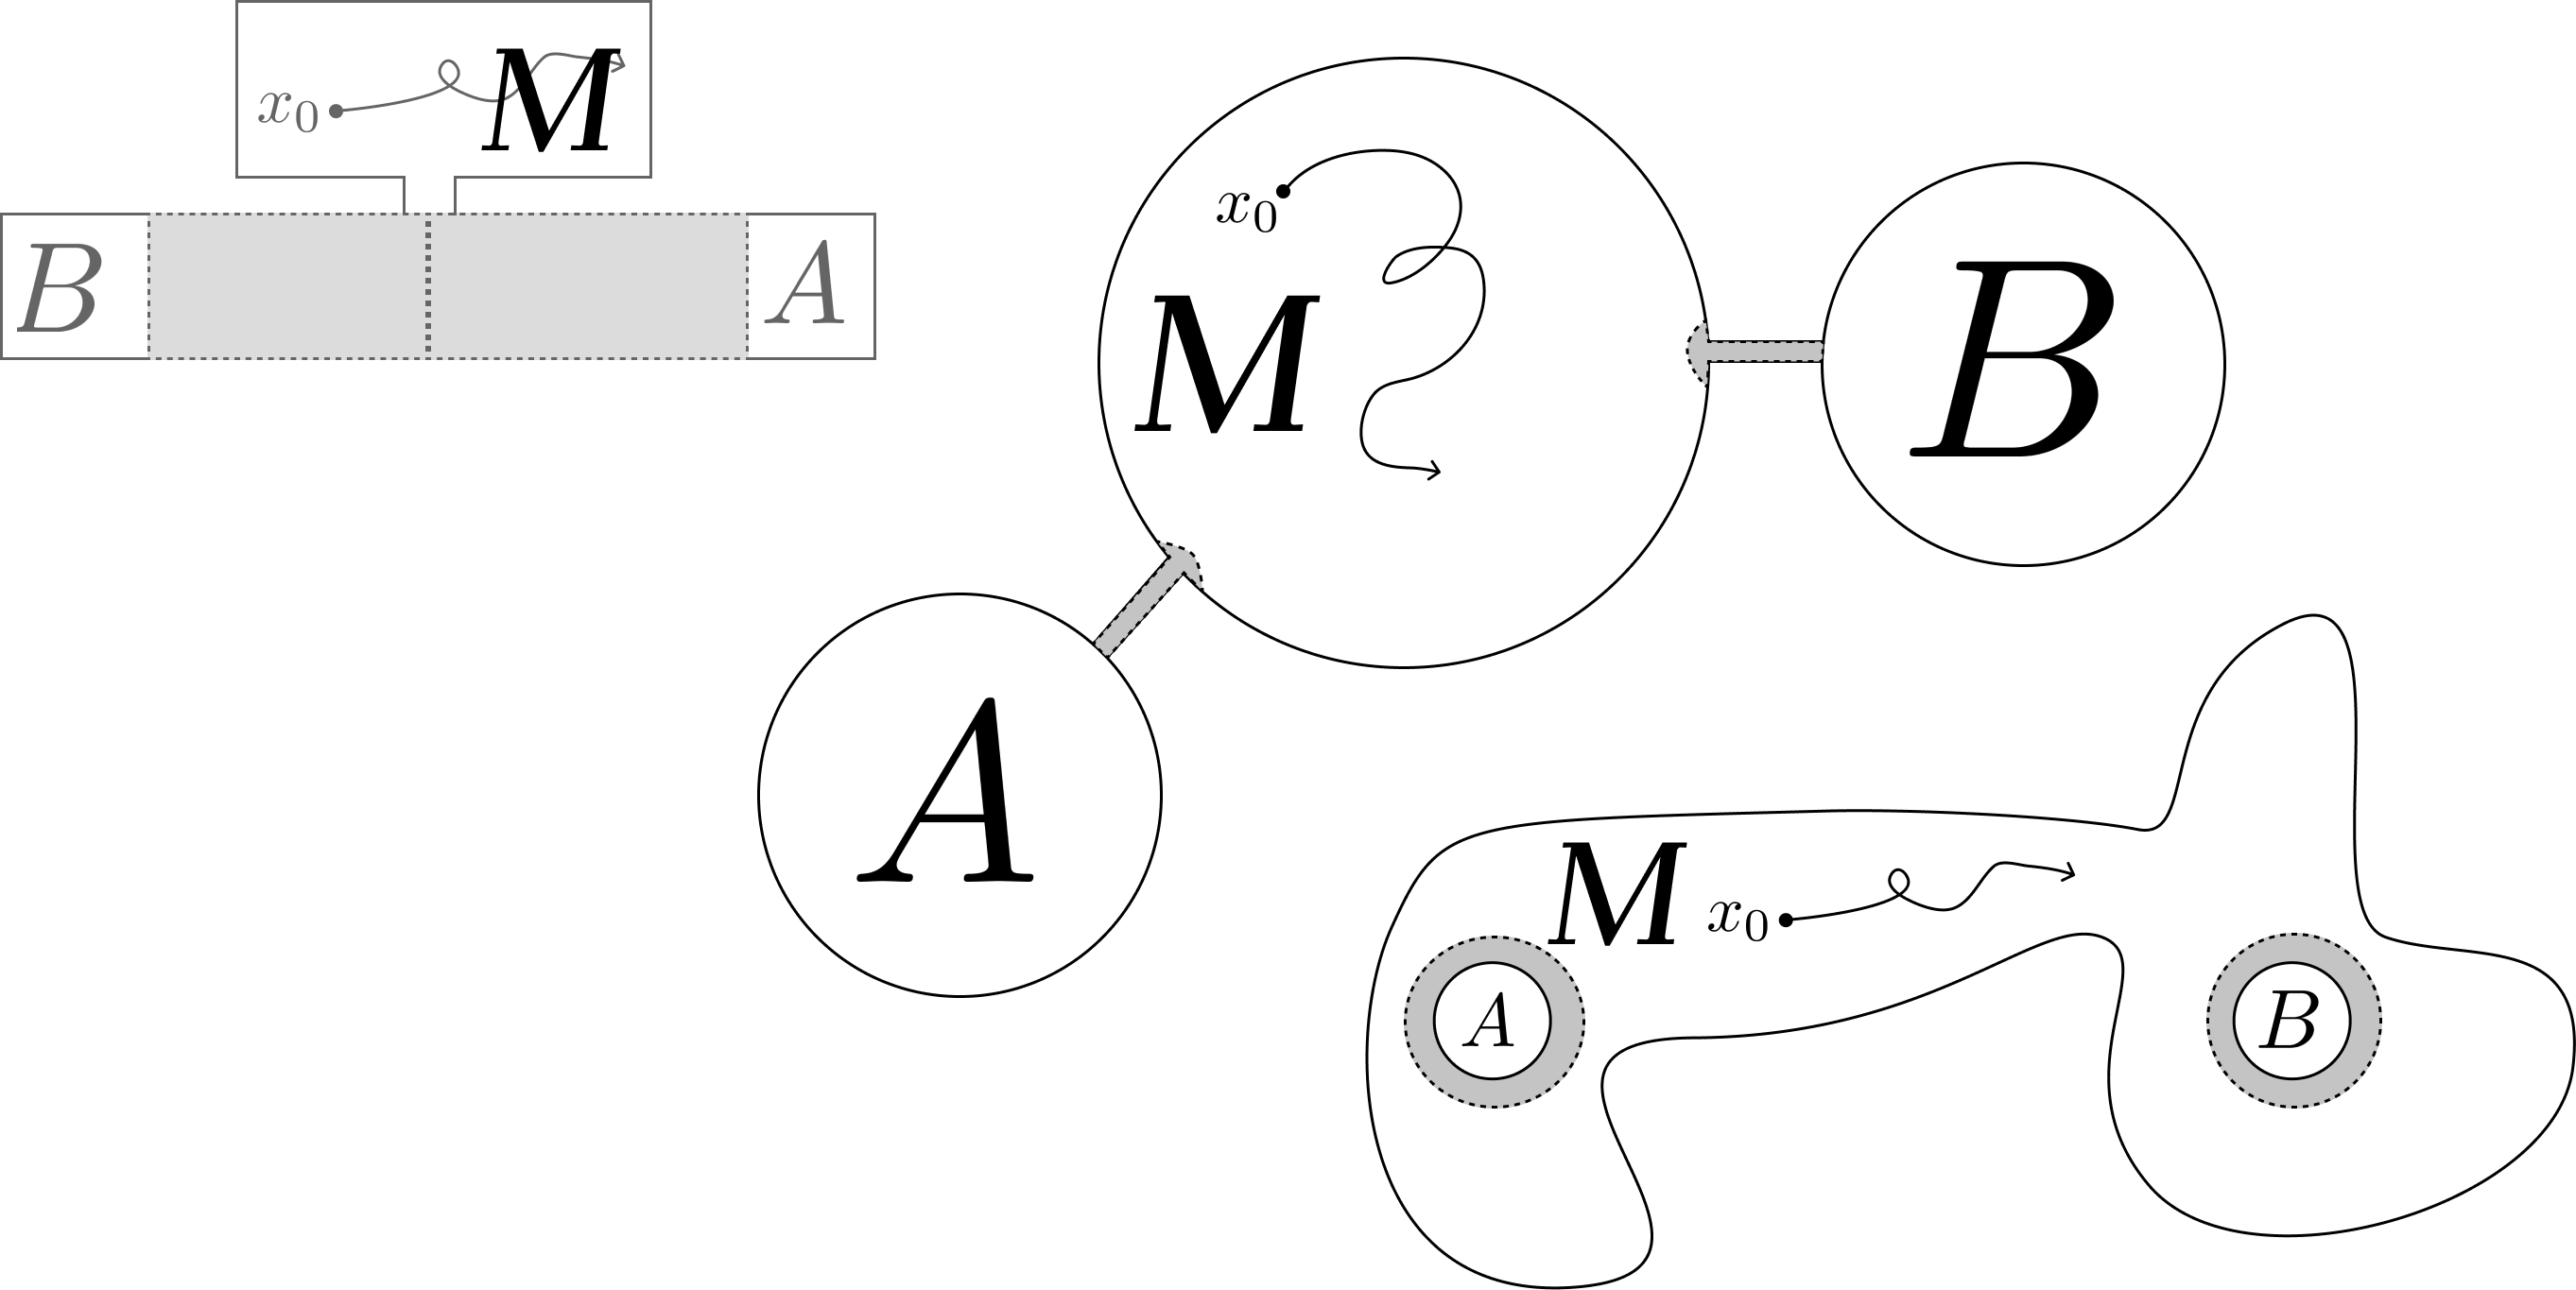
\includegraphics[width=0.8\textwidth]{bigpicture.png}
    \caption{\footnotesize\linespread{1.}\selectfont{} {\bf First passage capacities allow efficient computation of hitting probabilities.} We consider a reversible stochastic differential equation in an $n$-dimensional state-space, initialized at some configuration $x_0$ inside a set $M$. What is the probability that 
the diffusion will reach region $A$ before $B$?  We assume that the hitting probability is nearly the same for every initial condition $x_0 \in M$---differing by at most $\varepsilon$ 
across all initial conditions.  
(See Theorem \ref{thm:epsilon_flat} for some sufficient conditions, involving small targets and/or high dimensions.)
Theorem \ref{thm:main_thm} 
establishes an approximation to the hitting probability that
is accurate to within $\varepsilon + \sqrt{\varepsilon/2}$, and uses only ``first-passage capacities.'' These capacities can be computed from simulations that take place locally, meaning in the neighborhoods of the targets and entirely outside of $M$.  Here we depict several examples. In each case, the first-passage capacities can be computed efficiently using simulations confined only to the areas shaded in gray.}
\label{fig:ToyModel}
\vglue -1cm
\end{figure}


In the following section (\S\ref{sec:Preliminaries} ``Preliminaries'') we introduce notation, define the diffusion
and first-passage probabilities, enumerate the main assumptions, and finally define the first-passage capacities that are at the heart of this approach.  In \S\ref{sec:MainResults} we show that these capacities can be used to accurately estimate first-passage probabilities, and in way of examples, we give some sufficient conditions that guarantee that the main assumptions are satisfied. In \S\ref{sec:Estimation}, we develop the ``shell method,'' a numerical approach to computing first-passage capacities.   And in \S\ref{sec:Experiments} we investigate the speed and accuracy of the capacity-based approach in a variety of  
computational experiments.

\section{Preliminaries}
\label{sec:Preliminaries}

The results in this paper are about diffusion processes $X$ confined to an open bounded set $\Omega \subset \mathbb{R}^n$ with reflecting smooth boundary $\partial\Omega$ for $n\geq 3$.  We assume $X$ is driven by an $n$-dimensional standard Brownian motion $W$, i.e.
\begin{equation}\label{equ:general_sde}\mathrm{d} X_t = b (X_t) \mathrm{d} t + \sigma (X_t) \mathrm{d} W_t \end{equation}
where $b: \Omega \rightarrow \mathbbm{R}^n$ and $\sigma :
\Omega \rightarrow \mathbbm{R}^{n \times n}$ are continuously differentiable vector-valued and matrix-valued functions.  We further assume that $a(x)=\sigma(x)\sigma(x)^T$ is uniformly elliptic on $\Omega$, i.e. the smallest eigenvalues of $a$ are bounded away from zero.  Let $\bar \Omega$ denote the closure of $\Omega$ (and in general let $\bar S$ denote the closure of any set $S\subset \bar \Omega$).  For the precise definition of the reflected process, we adopt the framework developed by Lions and Sznitman\cite{lions1984stochastic}: Let $\normal=\normal(x)$ denote the outward normal of $\partial \Omega$ and $\nu:\ \partial \Omega \rightarrow \mathbb{R}^n$ a smooth vector field satisfying $\normal^T\nu\geq c>0$, and assume that $x_0 \in \Omega$.  Then there is a unique pathwise continuous
and $W$-adapted strong Markov process $X_t\in\bar\Omega$, and (random) measure $L$, such that
\begin{gather}\label{eq:SDER}
X_t = x_0 + \int_0^t b(X_s)ds + \int_0^t \sigma(X_s)dW_s - \int_0^t \nu(X_s) L(ds)
\end{gather}
and $L(\{t:\ X_t \notin \partial \Omega\})=0$.
For convenience, we will refer to $X$ by simply saying ``the reflected diffusion process (\ref{equ:general_sde}).'' We further assume that $X$ is a reversible process, with equilibrium distribution given by
\[
\rho(x)\doteq \frac{1}{Z}e^{-U(x)}\ \ \
Z=\int_{x\in\Omega}e^{-U(x)}dx
\]
where $U:\bar \Omega \rightarrow \mathbb{R}$ is continuously differentiable.  As shown by Chen \cite{chen1993reflecting}, to ensure that $X$ is reversible it is sufficient that
\begin{align}
\begin{split}
b_i(x)&=\frac{1}{2} \sum_j \partial a_{ij}(x)/\partial x_j - \frac{1}{2}\sum_j a_{ij}(x) \partial U(x)/\partial x_j
\label{eqn:reversibility} \\
\nu(x)&= a(x) \normal(x)
\end{split}
\end{align}
where $a(x)=\sigma(x)\sigma(x)^T$ is uniformly elliptic.
When the conditions in (\ref{eqn:reversibility}) are in force
we will say that $X$ satisfies the reversibility conditions relative to $U$.  We assume these conditions throughout the paper.

The main goal of this paper is to estimate first-passage  probabilities for $X$.  We here give a formal definition for these hitting probabilities for the two-target case, although all of our results extend, straightforwardly, to finite collections of targets:

\begin{definition}(First passage probabilities).  Fix two disjoint sets $A,B\subset \Omega$.  The first-passage probability function $h_{A,B}(x)$ is the probability that the process $X$ visits $A$ before $B$ if it is initialized at $X_0=x$.  Formally,
\[ h_{A, B}(x) \triangleq \mathbb{P}(X_{\tau_{A\cup B}}\in A|X_0=x)\]
where $\tau_{A\cup B}$ indicates the first-passage time to $A\cup B$, i.e.\ $\tau_{A\cup B} \triangleq \inf \{ t \geqslant 0 : X_t \in A \cup B \}$.  Throughout this paper we will use $\tau_S$ to denote the first-passage time to a set $S$ and $h_{S,S'}$ to denote the hitting probability function for targets $S,S'$.
\end{definition}

As discussed in the introduction, these hitting probabilities are much easier to estimate if the process forgets its initial condition to such an extent that the hitting probabilities are nearly constant for any initial condition inside a set $M$.  Here we give a formal definition for this property:
\begin{definition}(The $\varepsilon$-flatness condition)  A hitting probability function $h_{A,B}(x)$ is said to be
``$\varepsilon$-flat relative to $M$'' whenever
\[
\sup_{x, y \in M} |h_{A,B}(x) - h_{A,B}(y)| < \varepsilon
\]
\end{definition}
As we shall see in Theorem \ref{thm:main_thm}, this condition is exactly what we need to show that the hitting probabilities within $M$ can be well-approximated using ``first-passage capacities.''  These capacities are the last piece we must define:

\begin{definition}(Capacity)
Let $S \subset \tilde{S} \subset \Omega$ be open sets and let $X$ be a diffusion governed by the SDE in Equation (\ref{eq:SDER}) and satisfying the reversibility conditions in Equation (\ref{eqn:reversibility}).  The first-passage capacity $\ensuremath{\operatorname{cap}} (S, \tilde{S})$ for $X$ is defined as
%
\[ \ensuremath{\operatorname{cap}} (S, \tilde{S}) \triangleq \int_{\tilde S \backslash S}
||\sigma(x) \nabla h_{S, \tilde{S}^c}(x)||^2 e^{- U(x)} \mathrm{d} x \]
%
\end{definition}

We refer the reader to Appendix \ref{sec:three_perspectives} for more details on capacity and the related concept of Dirichlet form.  Note that there are several related definitions of ``capacity'' in the probabilistic potential theory literature, all slightly different.  For example, the harmonic capacity arises by taking the above definition in the special case when the diffusion is a simple Brownian motion.  The definition used here most closely follows the work of Bovier \cite{Bovier2016-ez,Bovier2004-wj}.  Throughout this work, the term is used only in the sense of the above definition.

\section{Main Theoretical Results}
\label{sec:MainResults}

Our main theorem shows that the first-passage capacities give accurate approximations of the hitting probabilities when the hitting probabilities are themselves $\varepsilon$-flat in a region outside a neighborhood of the targets.

\begin{theorem}\label{thm:main_thm}
Let $A\subset \tilde A,B\subset \tilde B$ be open sets and assume that  $h_{A,B}(x)$ is $\varepsilon$-flat relative to
$\Omega \backslash (\tilde A \cup \tilde B)$.
Then the first-passage probabilities are well-approximated by the first-passage capacities:
\[ \sup_{x \notin \tilde A,\tilde B} \left| h_{A,B} (x) - \frac{\capac{A}{\tilde A}}{\capac{A}{\tilde A}+\capac{B}{\tilde B}} \right| \leqslant \varepsilon + \sqrt{\varepsilon/2} \]
\end{theorem}

We defer the proof to Appendix \ref{sec:proof_thm}.  Note that the generalization to multiple targets is straightforward due to the additive property of capacities (Proposition \ref{prop:capacity} in Appendix \ref{sec:three_perspectives}).  In general, the hitting probability is approximately proportional to the corresponding capacity.

When might the $\varepsilon$-flatness condition hold?  In the introduction, we gave an intuitive explanation for when this might be expected to happen, namely whenever the diffusion forgets its initial condition before it hits the targets.  To prove the $\varepsilon$-flatness condition for a particular problem, one must make this idea rigorous. Here are two examples of how this might be done: 

\begin{theorem}\label{thm:epsilon_flat} (Examples of $\varepsilon$-flatness).   Let $\bb{x,r} = \{y:\ \Vert x-y \Vert < r\}$ denote the ball of radius $r$ centered at $x$.  Let us say that a diffusion governed by Equation (\ref{eq:pde}) ``behaves like Brownian motion'' on a set if $\sigma(x)=I$ and $\nabla U(x)=0$ for every $x$ in that set.  
\begin{enumerate}
    \item (small targets) Fix $r,\varepsilon>0$.  We can then find $\delta>0$ with the following property.  For any bounded convex set $\Omega$ with diameter less than or equal to 1, any $x_A,x_B \in \Omega$, any reversible stationary diffusion trapped inside $\Omega$ and behaving like Brownian motion for all $x\notin \bb{x_A, \delta} \cup \bb{x_B, \delta}$, and any $A\subset \bb{x_A, \delta}, B \subset \bb{x_B, \delta}$, we have that $h_{A,B}$ is $\varepsilon$-flat on $\Omega \backslash (\bb{x_A, r} \cup \bb{x_B, r})$.
    \item (high dimensions) Fix $r,\varepsilon>0$ and $r'<r$.  We can then find $n$ with the following property.  For any convex set $\Omega \in \mathbb{R}^n$ with diameter less than or equal to 1, any $x_A,x_B$ such that $\bb{x_A, r},\bb{x_B, r} \subset \Omega$, any reversible stationary diffusion trapped inside $\Omega$ and behaving like Brownian motion for all $x\notin \bb{x_A, r'} \cup \bb{x_B, r'}$, and any $A\subset \bb{x_A, r'}, B \subset \bb{x_B, r'}$, we have that $h_{A,B}$ is $\varepsilon$-flat on $\Omega \backslash (\bb{x_A, r} \cup \bb{x_B, r})$.
\end{enumerate}
\end{theorem}

A proof can be found in Appendix \ref{sec:proof_epsilon_flat}.  The first example shows how hitting probabilities become flat as the targets become small.  The second example notes that even if we fix the radius of the targets, the hitting probabilities becomes flat if the ambient dimension $n$ is high.  In both cases, the results are proved by showing that the rate of mixing inside $M$ is fast relative to the time it takes to exit $M$.

%      _          _ _                _   _               _ 
%  ___| |__   ___| | |_ __ ___   ___| |_| |__   ___   __| |
% / __| '_ \ / _ \ | | '_ ` _ \ / _ \ __| '_ \ / _ \ / _` |
% \__ \ | | |  __/ | | | | | | |  __/ |_| | | | (_) | (_| |
% |___/_| |_|\___|_|_|_| |_| |_|\___|\__|_| |_|\___/ \__,_|
                                                         


\section{Capacity Estimation via the Shell Method}
\label{sec:Estimation}
To make use of Theorem \ref{thm:main_thm} in practice, we must be able to compute capacities.  The calculation is local, in that $\capac{A}{\tilde{A}}$ is an integral on $\tA\backslash A$. We will propose here a Monte Carlo approach to evaluating the integral, using a combination of analytic reductions and local sampling. 

We begin by using an alternative formulation of the capacity:

\begin{proposition}
\label{prop:flux}
For any regions $G$ and $\tilde{G}$ having smooth boundaries and such that $A\subset G \subset \tilde G \subset \tilde A$, $\capac{A}{\tA}$ can be expressed as a flux leaving $\tilde G \backslash G$:
\begin{equation}
\label{eqn:GIntegral}
\ensuremath{\operatorname{cap}} (A, \tilde{A}) = \int_{\partial (\tilde G \backslash G)}  h_{A, \tilde{A}^c} (x)   \normal(x)^T a (x) \nabla h_{G, \tilde{G}^c} (x)e^{- U (x)} \hausdorffmeasure
\end{equation}
where $a(x)=\sigma(x)\sigma(x)^T$ is the diffusion matrix, $\hausdorffmeasure$ is the $(n-1)$-dimensional Hausdorff measure, and $\normal$ represents the outward-facing (relative to the set $\tilde G \backslash G$) normal vector on $\partial (\tilde G \backslash G)$.
\end{proposition}
\noindent (Results like this are well known, though perhaps not in exactly this form. In any case, we have included a formal proof which can be found in Appendix \ref{sec:proof_proposition}.)

There is a great deal of freedom in choosing $G$ and $\tilde G$; the idea is to choose them so as to make the surface integrals as simple as possible.  Each of these surface integrals can be viewed as an expectation.  Let $\hausdorffmeasure$ denote the $n-1$-dimensional Hausdorff measure.  We can define a probability measure on
$\partial G$ by
\[
\PMeasure\doteq\frac{1}{Z}e^{-U(x)}\hausdorffmeasure
\text{   where   }
Z= \int_{\partial G} e^{-U(x)}\hausdorffmeasure
\]
We can define $\tPMeasure$
and $\tilde{Z}$ analogously, on $\partial\tilde{G}$ rather than $\partial G$.
Then
\begin{align}
\capac{A}{\tilde A} & = \int_{\partial\tilde{G}} h_{A, \tilde{A}^c}    \normal^T a  \nabla h_{G, \tilde{G}^c} e^{- U } \hausdorffmeasure
-\int_{\partial G} h_{A, \tilde{A}^c}    \normal^T a  \nabla h_{G, \tilde{G}^c} e^{- U } \hausdorffmeasure
\nonumber \\
&=\tilde Z
\int_{\partial\tilde{G}} h_{A, \tilde{A}^c}    \normal^T a  \nabla h_{G, \tilde{G}^c} \tPMeasure
-Z
\int_{\partial G} h_{A, \tilde{A}^c}    \normal^T a
\nabla h_{G,\tilde{G}^c} \PMeasure
\label{eqn:PMeasureInt}
\end{align}
where, in these integrals, the normal, $\normal$, points outward from both $G$ and $\tilde G$.
Let $y_1,y_2,\dots,y_m\sim \text{iid}\ \PMeasure$, so that
\begin{align*}
\frac{1}{m}\sum_{i=1}^m
h_{A, \tilde{A}^c}(y_i) \normal^T(y_i) a(y_i)  \nabla h_{G,\tilde{G}^c}(y_i) & \stackrel{m\to\infty}{\longrightarrow}
 \int_{\partial G} h_{A, \tilde{A}^c}    \normal^T a
\nabla h_{G,\tilde{G}^c} \PMeasure \\
\text{and}\ \ \ \ \ \ \frac{1}{m}\sum_{i=1}^m e^{U(y_i)}
& \stackrel{m\to\infty}{\longrightarrow} \int_{\partial G} e^U
\PMeasure = \frac{|\partial G|}{Z}
\end{align*}
where $|\partial G|$ is the surface area of $G$. Putting these together, we get the large $n$ approximation
\[
Z
\int_{\partial G} h_{A, \tilde{A}^c}    \normal^T a
\nabla h_{G,\tilde{G}^c} \PMeasure
\approx
|\partial G|
\frac{\sum_{i=1}^m
h_{A, \tilde{A}^c}(y_i) \normal^T(y_i) a(y_i)  \nabla h_{G,\tilde{G}^c}(y_i)}
{\sum_{i=1}^m e^{U(y_i)}}
\]
If we now extend all of this to $\partial\tilde{G}$, with
$\tilde{y}_1,\tilde{y}_2,\dots,\tilde{y}_n\sim \text{iid}\ \tPMeasure$, and put the approximations into
(\ref{eqn:PMeasureInt}), then for large $n$ and $m$
\begin{align}
\capac{A}{\tilde A} & \approx
|\partial\tilde{G}|
\frac{\sum_{i=1}^n
h_{A, \tilde{A}^c}(\tilde{y}_i) \normal^T(\tilde{y}_i) a(\tilde{y}_i)  \nabla h_{G,\tilde{G}^c}(\tilde{y}_i)}
{\sum_{i=1}^n e^{U(\tilde{y}_i)}}
\label{eqn:approximate_capacity}\\
& -|\partial G|
\frac{\sum_{i=1}^m
h_{A, \tilde{A}^c}(y_i) \normal^T(y_i) a(y_i)  \nabla h_{G,\tilde{G}^c}(y_i)}
{\sum_{i=1}^m e^{U(y_i)}}
\nonumber
\end{align}

In summary: we can use a Monte-Carlo technique to compute the capacity as long as we can (i) sample from $\PMeasure$ and $\tPMeasure$; (ii) compute the surface areas $|\partial G|$ and
$|\partial\tilde{G}|$; (iii)
compute the first-passage probability $h_{A, \tilde{A}^c}$; and (iv) compute the gradient
$\nabla h_{G, \tilde{G}^c}$.  
We can often make tasks (i) and (ii) straightforward by a judicious choice of $G,\tilde G$.  However, tasks (iii) and (iv) are more difficult.  

Thus, to compute the capacity using this approach, the most difficult challenge is to compute the first-passage probabilities along $G,\tilde G$.  Broadly speaking there are two approaches for this kind of problem.  First-passage probabilities satisfy an elliptic PDE related to the infinitesimal generator -- see Appendix \ref{sec:three_perspectives}, Equation (\ref{eq:pde}) -- and we could therefore choose from a selection of numerical solvers. Here, in a different direction, we exploit the connection between first-passage probabilities and the underlying random walk in order to develop Monte Carlo tools suitable for estimating both $h_{A, \tilde{A}^c}$ and $\nabla h_{G, \tilde{G}^c}$ on the surfaces
$\partial G$ and $\partial\tilde{G}$. These tools are based on
what we will call the ``shell method,'' which we describe briefly in the following paragraphs and in full detail in Appendix \ref{sec:shell_method}.

Generically, given two simply-connected regions $R$ and $\tilde{R}$, with $R\subset \tilde{R}$, and a set $S$ such that
$R\subset S  \subset\tilde{R}$, we seek an approximation to
the function $h_{R,\tilde{R}^c}$ on the surface $\partial S$. In principle, we could begin with a fine-grained partitioning of $\partial S$ into simply-connected ``cells,'' and for each cell simulate the diffusion many times, recording whether or not the path first exits $\partial (\tilde{R}\backslash R)$ at $\partial R$. The fraction of paths that first exit at $\partial R$ constitutes an estimate of
$h_{R,\tilde{R}^c}(x)$ for any $x$ in the current cell. But this is wasteful and likely infeasible in all but the simplest of settings. Much of the waste stems from the fact that the ensemble of all paths generated from all cells will likely include many near collisions of paths scattered throughout $\partial (\tilde{R}\backslash R)$. An alternative, divide-and-conquer  approach, is to introduce multiple sets, $S_0,S_1,\ldots,S_n$ such that
\begin{equation*}
R=S_0 \subset \cdots \subset S_{m-1}\subset S_m = S \subset S_{m+1} \subset \cdots \subset S_n = \tilde{R}
\end{equation*}
and use sample paths from $X$, {\em locally}, to estimate the transition probability matrices from each cell within each ``shell'' $\partial S_k$ to each cell of its neighboring shells, $\partial S_{k-1}$ and $\partial S_{k+1}$. Equipped with these transition matrices, the first-passage probability for a given $x\in S$ is computed algebraically, without further approximation.

$S$ must have been chosen not only to satisfy $R\subset S  \subset\tilde{R}$ but also in such a way as to make it feasible to sample from $\partial S$ under the probability measure
$\frac{1}{Z}e^{-U}\hausdorffmeasure$. After that, $S_k\ k=1,\ldots,n-1$ are chosen so that the shells nest and are in close proximity; the hitting times starting from a sample in $\partial
 S_k$ and ending at $\partial S_{k-1} \cup \partial S_{k+1}$ must be short enough to encourage many repeated runs. The output is a set of samples,
 $z_1,\ldots,z_N \sim \frac{1}{Z}e^{-U}\hausdorffmeasure$ on $\partial S$ together with the approximate value of $h_{R,\tilde{R}^c}(x)$ at each sample $x=z_i$. (In fact, though the main purpose is to estimate $h_{R,\tilde{R}^c}$ on
 $\partial S$, a byproduct is a sample from $\frac{1}{Z}e^{-U}\hausdorffmeasure$ on all of the shells $\partial S_k$, along with an estimate of $h_{R,\tilde{R}^c}$ at every sample.)
With the choice of $A$ for $R$ and $\tilde A$ for $\tilde R$, the algorithm becomes directly applicable to the estimation of $h_{A, \tilde{A}^c}$ on $\partial G$ and $\partial\tilde{G}$, taking $S=G$ in the former case and $S=\tilde{G}$ in the latter.

The shell method is closely related to milestoning\cite{West2007-cn, Bello-Rivas2015-ld, Aristoff2016-gc} and Markov state models\cite{Pande2010-yi, Chodera2014-bh, Husic2018-xp}, though more tailored to the problem at hand. In particular, our interest here is in computing the first-passage probabilities rather than in approximating the underlying process. Also, the discretizations of the shells are {\em adaptive}, in that they are based on clusters that are derived from an ensemble of samples, as opposed to being crafted for a particular landscape.  See Appendix \ref{sec:shell_method}.

As for the required gradients, these are generally harder to estimate. Nevertheless, for the particular gradient $\nabla h_{G, \tilde{G}^c}$, the problem is substantially mitigated by noting that we are only interested in its evaluation on $\partial G$ and $\partial\tilde G$, each of which is a level set of
$h_{G, \tilde{G}^c}$ ($h_{G, \tilde{G}^c}=1$ on $G$ and 0 on $\tilde G$). Consequently, on each surface the gradient is in the normal direction and we need only estimate its magnitude. And for this purpose it is enough to know the values of $h_{G, \tilde{G}^c}$ on a surface close to $G$ and interior to $\tilde{G}\backslash G$ (for estimating $\nabla h_{G, \tilde{G}^c}$ on $G$) and on another surface
close to $\tilde{G}$ and also interior to $\tilde{G}\backslash G$ (for estimating $\nabla h_{G, \tilde{G}^c}$ on $\tilde G$). Two such surfaces would be $\partial S_1$ and $\partial S_{n-1}$, were we to apply the shell method with $R=G$ and $\tilde{R}=\tilde{G}$,
since, as already noted, a byproduct of the method is an estimate of
$h_{R,\tilde{R}^c}$ on all of the shells. Alternatively, in the interest of better accuracy, the method could be run twice, once with $S=S_1$, a well-chosen outer approximation of $G$, and then again with
$S=S_{n-1}$, a well-chosen inner approximation of $\tilde G$.

%%%%%%%%%%%%%%%%%%%%%%%%%%%%%%%%%%%
%%%%%%%%%%%%%%%%%%%%%%%%%%%%%%%%%%%
%%%%%%%%%%%%%%%%%%%%%%%%%%%%%%%%%%%
%%%%%%%%%%%%%%%%%%%%%%%%%%%%%%%%%%%

%                                  _           _                       _ _       
%  _ __  _   _ _ __ ___   ___ _ __(_) ___ __ _| |  _ __ ___  ___ _   _| | |_ ___ 
% | '_ \| | | | '_ ` _ \ / _ \ '__| |/ __/ _` | | | '__/ _ \/ __| | | | | __/ __|
% | | | | |_| | | | | | |  __/ |  | | (_| (_| | | | | |  __/\__ \ |_| | | |_\__ \
% |_| |_|\__,_|_| |_| |_|\___|_|  |_|\___\__,_|_| |_|  \___||___/\__,_|_|\__|___/
                                                                               


\section{Numerical Experiments\footnote{All the experimental results can be reproduced or easily modified from open-source code, which can found, along with detailed instructions, at \url{https://github.com/StannisZhou/entropic_barrier}.}}\label{sec:Experiments}
%We use numerical experiments to test the practical relevance of our theoretical results and capacity-estimation algorithm.  There several questions we would like to address empirically:
We used a series of experiments to investigate 
the accuracy and computational efficiency of the proposed
approach to estimating first-passage probabilities. Three 
questions were addressed empirically, in each of several settings:

\begin{itemize}

\item Is the first-passage probability function 
 $\varepsilon$-flat?  
The capacity approach to first-passage probabilities (Theorem  \ref{thm:main_thm}) is predicated on the assumption that 
$h_{A,B}(x)$ is $\varepsilon$-flat over a region that is sufficiently removed from the immediate neighborhoods of the targets.
Theorem \ref{thm:epsilon_flat} gives asymptotic (small-target or high-dimension) sufficient conditions. How quickly do these asymptotic limits come into play?  We estimated, numerically, the extent of $\varepsilon$-flatness in each setting. 
	
\item How tight are the bounds in Theorem \ref{thm:main_thm}?  The Theorem guarantees that the first-passage probability function is within $\theepsrate$ of the probability determined by the target-capacity ratios.  We estimated the tightness of the bound in each setting. 

\item Is the shell method accurate and computationally efficient?  
Target capacities can rarely be computed analytically, and hence the applicability of the capacity-based approach to first-passage probabilities depends upon the accuracy and computational efficiency of the shell method (\ref{sec:Estimation}).  We examined both in each of many settings. 
\end{itemize}

We looked at problems of the following form.  In every case the configuration space,
$\Omega$, was the unit ball in $\mathbb{R}^5$.  In other words, 
$\Omega = \bb{0,1}$, where $\bb{x, r} \triangleq \{ y : || y - x || < r \}$. The diffusion was confined to $\Omega$ by a reflecting boundary at $\partial\Omega$, and within $\Omega$ the dynamics were assumed to obey the first-order (high-viscosity) Langevin equation,
\begin{equation}
\label{equ:toy_sde}
\mathrm{d} X_t = - \nabla U (X_t) \mathrm{d} t + \mathrm{d} W_t
\end{equation}
where $W_t$ is an $n$-dimensional Brownian motion and
$U$ is a potential energy. Although the method applies to multiple targets (as noted earlier), the experiments involved only  two,
\begin{align*}
A &\triangleq \bb {x_A, r_A}\\
B &\triangleq \bb {x_B, r_B}
\end{align*}

Given an initial condition $X_0\in \Omega \backslash (A\cup B)$, we are interested to know whether the dynamics carry the system into $A$ or $B$ first.  We further assumed that $U$ is constant beyond the immediate neighborhoods of $A$ and $B$: letting $\dA=\bb{x_A,r_\dA }$ and $\tA=\bb{x_A,r_\tA }$ such that $r_A<r_\dA<r_\tA$, and letting $\dB=\bb{x_B,r_\dB }$ and  $\tB=\bb{x_B,r_\tB}$ such that $r_B<r_\dB<r_\tB$, we assumed that $\nabla U(x)=0$ for all $x\in\Omega\backslash (\dA\cup\dB)$.  Our interest is in estimating $h_{A,B}(x)$ over the region $x=X_0 \in \Omega\setminus \tA \cup \tB$.  

In order to establish good estimates for ground truth, 
we ran a total of 400,000 simulations of (\ref{equ:toy_sde}) 
until the first passage to $A$ or $B$, 
in each of six experiments. This was greatly facilitated by
the assumption that
 $\nabla U(x)=0$ outside of $\dA\cup\dB$, since we could use
 the ``walk-on-spheres'' method (cf.\ \cite{bingham1972random})
for the corresponding portions of the trajectory.

We considered two broadly different variations of the set-up: one (Brownian diffusion) in which the
{\em exact} target capacities could be computed, thereby allowing for a direct assessment of the accuracy of the shell method,  and the other involving complex energy landscapes in the neighborhoods of the targets. In the latter case, the accuracy of the capacity estimates could only be inferred from the accuracy of the resulting estimates of first-passage probabilities.

\subsection{Brownian Diffusion}
\label{sec:B_D}

\begin{figure}
\fbox{\begin{minipage}{\textwidth}
    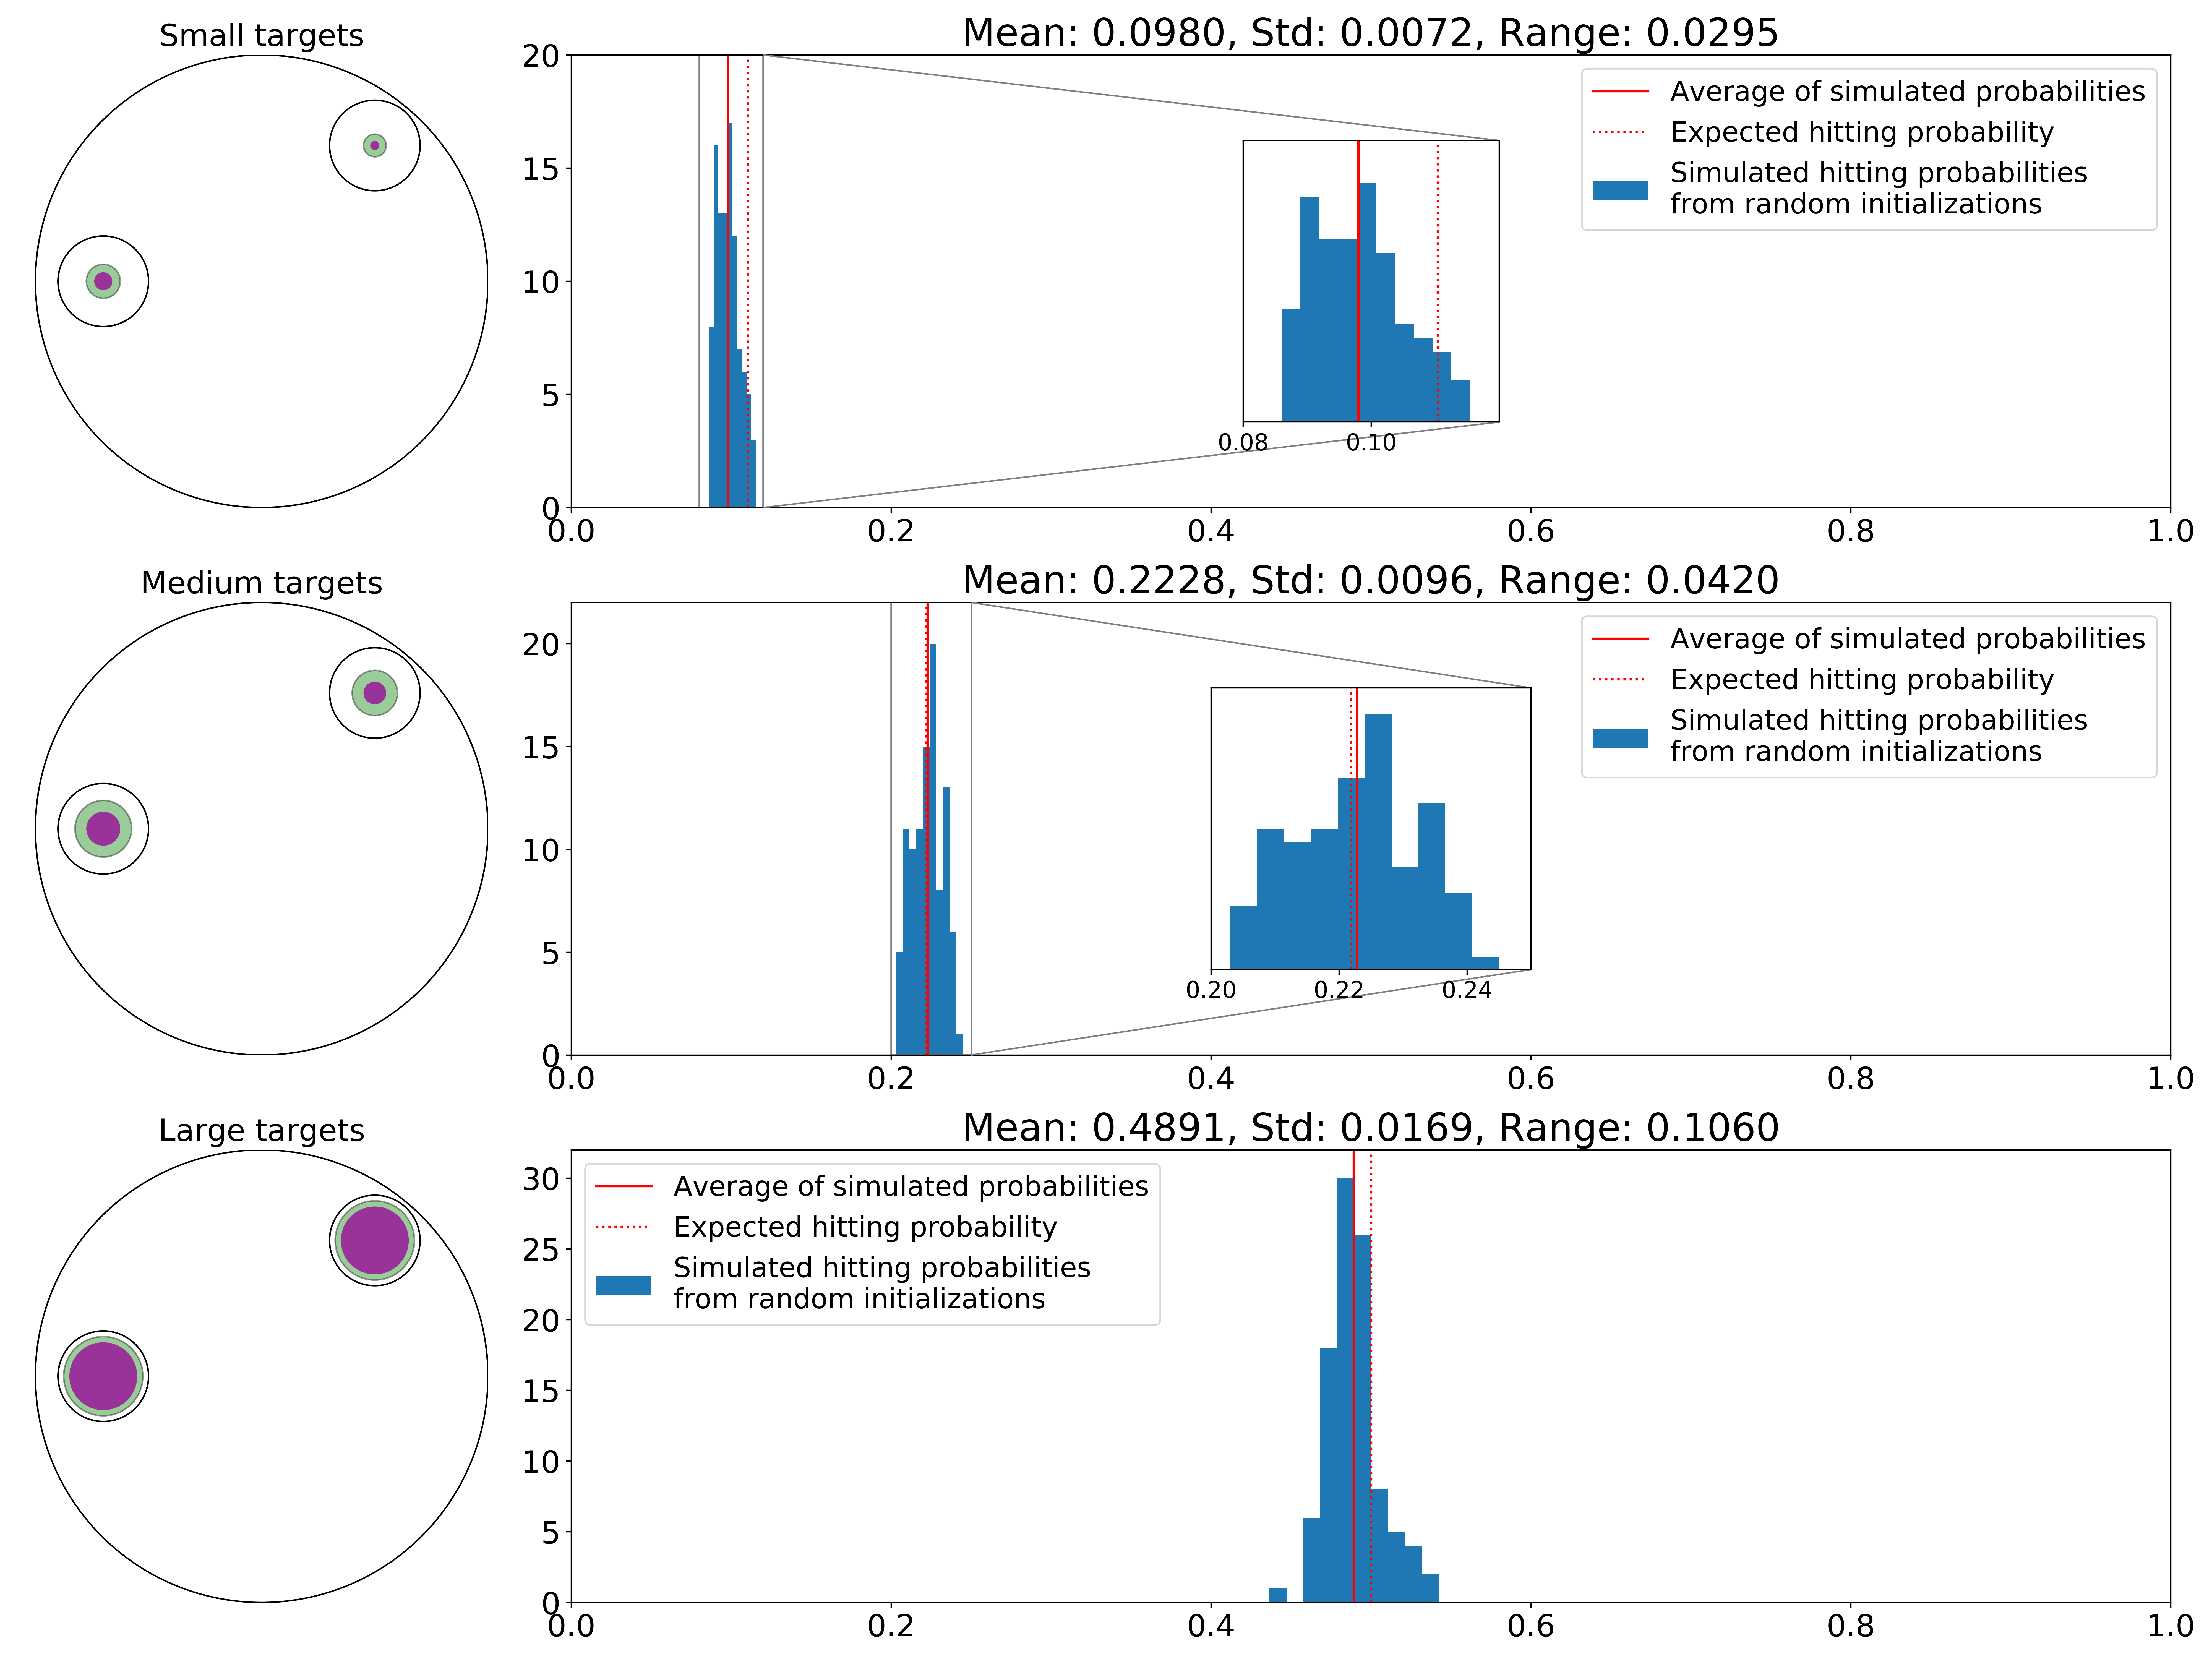
\includegraphics[width=\textwidth]{results_brownian_motion.png}
    \caption{\label{fig:results_brownian_motion}{\bf 
    Capacities and first-passage probabilities: Brownian motion.}
We consider three different cases (small, medium and large), as illustrated in the left side of the figure.  In each case we have two targets and are interested in the probability that a Brownian motion will first encounter target $A$ before target $B$.  We consider 100 random initial locations,  confined to be outside of the small black circles. For each location, we use 2,000 runs of the diffusion to estimate the probability of hitting target $A$ before $B$.   We plot these 100 estimates as a histogram.  The histograms reveal that the hitting probabilities fall within a narrow range, especially when the targets are small.  Moreover, we see that the location of this narrow range can be accurately predicted by the capacity-based approximation in Theorem \ref{thm:main_thm} ($p_A$ from equation \ref{eqn:p_A},
shown as a dotted red line); the capacity-based approximation, derived from purely {\em local} computations within the neighborhoods of the targets, always falls inside the span of the histogram.  We can further compare the capacity-based value to an estimate of the mean hitting probability for a process initialized at a random location, which is just the relative frequency of hitting $A$ before $B$ in  200,000 additional simulations from random initial conditions (shown as a  solid red line.)}
\end{minipage}}
\end{figure}

The first set of experiments tested the capacity-based approach in the simplest possible case: $U(x)=0$ for all $x$ outside of the targets. The target centers were fixed
at $x_A=(0.5,0.6,0.0,0,0,0.0)$ and $x_B=(-0.7,0.0,0.0,0,0,0.0)$, the radii $r_\tA$ and $r_\tB$ were fixed at $0.2$, 
and the radii $r_A$ and $r_B$ were varied across three conditions. These were defined as ``small targets'' ($r_A=0.02, r_B=0.04$), ``medium targets'' ($r_A=0.05, r_B=0.075$) and ``large targets'' ($r_A=r_B=0.15$). 
The three cases are illustrated, along with the corresponding results, in Figure \ref{fig:results_brownian_motion}.  
(In light of the assumption $U(x)=0$, the particular values of
$r_\dA$ and $r_\dB$ 
are irrelevant in this set of experiments, though not in the next set---see \ref{sec:nontrivial_results}.)

Each of the three questions raised earlier 
(Is the first-passage probability function 
 $\varepsilon$-flat?
 How tight are the bounds in Theorem \ref{thm:main_thm}? 
 Is the shell method accurate and computationally efficient? )
was explored for each of the three target sizes.  

\subsubsection{Is the first-passage probability function 
 $\varepsilon$-flat?}
\label{sec:toy_constant}
Theorem \ref{thm:epsilon_flat}, although an asymptotic result, suggests that the variability of the first-passage probabilities will decrease with target size. 
To investigate this relationship we conducted 2,000 diffusion simulations at each of 100 randomly selected initial conditions,
$X_0 \in \Omega\setminus \tA \cup \tB$.  These simulations yielded 100 well-estimated hitting probabilities.  The histograms of these probabilities are displayed in Figure \ref{fig:results_brownian_motion}.  As the targets become smaller, the histograms become more peaked.  
A crude estimate of the flatness of $h_{A,B}(x)$ is the 
spread of the 100 estimated probabilities:
\begin{itemize}
    \item $\varepsilon\approx 0.0295$ for the small targets
    \item $\varepsilon\approx 0.0420$ for the medium targets
    \item $\varepsilon\approx 0.1060$ for the large targets
\end{itemize}
In other words, the dependency of the hitting probability on the initial condition decreases with target size, as anticipated.


\subsubsection{How tight are the bounds in Theorem \ref{thm:main_thm}?}
\label{sec:toy_capacity}
If we were to take these estimates of $\varepsilon$-flatness and apply Theorem \ref{thm:main_thm}, as though they were precise measurements, then we would conclude that 
\begin{equation}
\label{eqn:bound}
\sup_{x \notin \tilde A,\tilde B} \left| h_{A,B} (x) -p_A
\right| \leqslant \varepsilon + \sqrt{\varepsilon/2} 
\end{equation}
where 
\begin{equation}
\label{eqn:p_A}
p_A\triangleq 
   \frac{\capac{A}{\tilde A}}{\capac{A}{\tilde A}+\capac{B}{\tilde B}}  
\end{equation}
and $\varepsilon +
\sqrt{\varepsilon/2}=0.0295+\sqrt{0.0295/2}
\approx 0.15$ for the small targets, and 0.19 and 0.34 for the medium and large targets, respectively.

In this special case, in which the diffusion is just a Brownian motion outside of the targets, the capacities can be computed exactly via the formulas
\begin{equation}
\label{eqn:analytic_capacities}
\capac{A}{\tA}  =
\frac{6\pi^{\frac{5}{2}}}
{\Gamma(\frac{5}{2})(r_A^{-3} - r_\tA^{-3})}  \qquad
\capac{B}{\tB}  =
\frac{6\pi^{\frac{5}{2}}}
{\Gamma(\frac{5}{2})(r_B^{-3} - r_\tB^{-3})}
\end{equation}
which are easily derived using the representation in equation (\ref{eqn:GIntegral}), established in Proposition \ref{prop:flux}. Together with (\ref{eqn:p_A}), we then get the following formula for the corresponding probabilities:
\begin{equation*}
p_A = \frac{\frac{1}{r_A^{-3} - r_{\tilde{A}}^{-3}}}{\frac{1}{r_A^{-3} - r_{\tilde{A}}^{-3}} + \frac{1}{r_B^{-3} - r_{\tilde{B}}^{-3}}}
\end{equation*}
which evaluates to 0.1104, 0.2219, and 0.5, respectively for the small, medium and large targets. These capacity-based estimates are indicated in Figure \ref{fig:results_brownian_motion} by the dotted red lines, which are  superimposed on the corresponding histograms of the one-hundred empirically derived probabilities.

To the extent that the range of the 100 well-estimated hitting probabilities (2,000 samples of the diffusion starting at each of the 100 randomly selected starting locations) is a reasonable estimate of the $\varepsilon$-flatness, for a given pair of targets,
we are now in a position to evaluate the accuracy of the bound guaranteed by Theorem {\ref{thm:main_thm}, i.e. the bound in equation (\ref{eqn:bound}). In particular, in each of the three examples depicted in Figure \ref{fig:results_brownian_motion}
the value of $p_A$ (dotted red line) lies within the range of the corresponding histogram. Therefor, in each of the three examples,  the maximum error is smaller than our estimate of $\varepsilon$ itself. For these examples, the theoretical bound appears to be fairly loose---in each case  $\varepsilon +
\sqrt{\varepsilon/2}$  could be replaced by  $\varepsilon$, which comes to 0.0295 instead of 0.15 for the small targets, and 0.0420 instead of 0.19 and 0.1060 instead of 0.34 for the medium and large targets. Possibly, the {\em asymptotic} bound ($\varepsilon\to
0$), which is not addressed by Theroem \ref{thm:main_thm},
is dominated by $\varepsilon$ rather than $\sqrt{\varepsilon}$.


\subsubsection{Is the shell method accurate and computationally efficient?}
\label{sec:toy_shell}
As noted in \S\ref{sec:toy_capacity}, the special assumptions in these examples allow us to compute the exact capacities, according to equation (\ref{eqn:analytic_capacities}). Hence we can directly measure the accuracy of the approximations computed with the shell method.\footnote{With reference to Appendix \ref{sec:shell_method}, the following parameters were used to implement the shell method: $m = 2, n = 4, N_p = 100, N_b = 3, N_s = 1000$, and a time-step of $10^{-7}$.}
Table \ref{table:brownian_capacities} summarizes the results for
each of the three target sizes. 
By Theorem \ref{thm:main_thm}, the capacities enter into an approximation of first-passage probabilities through $p_A$, 
as defined in equation (\ref{eqn:p_A}). 
The third and fourth rows of the table give the exact values of $p_A$ and the corresponding values derived from the shell-estimated capacities, respectively. The differences are small relative to the spread of first-passage probabilities and, in particular, each of the estimated values lies comfortably within the range of estimated probabilities (cf. Figure 
\ref{fig:results_brownian_motion}).
The shell method does not introduce any significant additional error for these problems.


\begin{table}[!ht]
\begin{tabular}{ c| c c c}
      Targets & small & medium & large  \\
  \hline
  $\large(\capac{A}{\tilde A},\capac{B}{\tilde B}\large)$ 
  & (0.000632,0.005094) 
  & (0.010026,0.035164)
  & (0.460937,0.460937)
   \\
$\large(\hatcapac{A}{\tilde A},\hatcapac{B}{\tilde B}\large)$
  &(0.000549,0.004699)
  &(0.009308,0.033625)
  &(0.452441,0.451537)
  \\
  $p_A$ & 0.1104 & 0.2219 & 0.5000\\
  $\hat{p}_A$  & 0.1091 &0.2168 & 0.5005 \\
  \end{tabular}
  \caption{{\bf Accuracy of the shell method: Brownian motion.} 
  There are thee pairs of targets, labeled small, medium and large.
 The target capacities, which can be calculated exactly for Brownian motion, are entered in the first row. The second row contains the corresponding estimates derived by the shell method
(cf. \S\ref{sec:Estimation}). According to Theorem \ref{thm:main_thm}, $p_A$ (\ref{eqn:p_A}) is an estimate of the probability that the first passage occurs at $A$, accurate to within an error of $\varepsilon$ + $\sqrt{\varepsilon/2}$. The exact values
 of $p_A$ are entered in the third row, and the estimated values, derived from the estimated capacities, are in the fourth row.}
\label{table:brownian_capacities}
\end{table}

Turning now to the question of computational efficiency, 
how fast is a capacity-estimation approach when compared against a simulation-based approach?  There are of course many
variables that might affect the comparison, including the dimension and the details of the energies, not to mention the implementation details. In our experiments with direct simulations, we used the ``walk-on-spheres'' method to simulate trajectories in the flat region \cite{bingham1972random}, JIT compilation to remove loop overhead, multi-CPU parallelization, and the coarsest time step that yielded accurate results. (In that the walk-on-spheres method requires a flat energy landscape and Theorem \ref{thm:main_thm} does not, 
our inferences about computational efficiency are, in this regard, somewhat tilted in favor of the simulation approach.)
As for capacity estimation, we made no effort to adjust the number of samples or the discretization parameters. 

In both the Brownian-motion experiments discussed in this section and the experiments with non-trivial landscapes discussed in the next section, we observed that a single run of direct simulation took about as long as estimating two capacities using the shell method,
i.e. as long as it takes to compute the capacity-based estimate of the first-passage probability. With this benchmark in hand, the comparison of the two approaches comes down to the question of accuracy: How many direct simulations would be needed to compute the first-passage probability to within an accuracy 
comparable to what was obtained using capacities? 

A single simulation run produces  a single Bernoulli variable---one if target $A$ is encountered before target $B$, and zero otherwise. The total number of ones, then, in a sequence of independent simulations will have a binomial distribution. Hence, given any probability $p$ of the Bernoulli event ``one,''
and any desired accuracy $\delta$, the number of independent simulations needed to achieve a confidence interval of size $\delta$, with 95\% confidence, is
about $n(\delta)=4\frac{p(1-p)}{\delta^2}$.\footnote{
In principle, the value of $p$ depends on the starting location. But in light of the tight clustering of first-passage probabilities ($\varepsilon$-flatness), we used the mean value obtained from 200,000 samples at random starting locations, which is designated ``Mean of simulated probabilities'' in the figures, 
for all calculations of sample sizes.}
Since a single simulation run takes about as long as our capacity-based estimation for $p_A$, we can assert that in this sense the capacity-based estimation is approximately $n=n(\delta)$ times more efficient.

What is a reasonable value of $\delta$? Here are two points of view, leading to similar estimates of $n$:
\begin{enumerate}
\item 
Let $\hat{p}_A$ be the capacity-based estimate 
of first encountering $A$ after starting at a given location 
$x \in \Omega\setminus \tA \cup \tB$
(indicated, for each of the three experiments, by the dotted red line in Figure
\ref{fig:results_brownian_motion}), 
and recall that $h_{A,B}(x)$ 
represents the actual probability, which in general depends on the starting location, $x$.
Keep in mind that the capacity-based estimator is independent of $x$. If the starting location were chosen randomly, then an unbiased estimator of the mean absolute error,
$\mathbb{E}[| h_{A,B}(X) - \hat{p}_A |]$, 
for a given value of $\hat{p}_A$,
is obtained by taking expectation with respect to the empirical probability distribution, which is displayed in the figure by a histogram for each target size.
The resulting three estimates, for the small, medium, and large targets, of the mean absolute errors are 
0.0127,
0.0080,
and 0.0167, respectively. 
From this point of view (i.e. using these three values for $\delta$),
{\em 
the number of simulation runs from a given location $x$ needed to achieve an error approximately equal to the mean absolute error of the capacity method, and hence the computational advantage of the capacity method, is about 
2,000 for the small targets, 10,000 for the medium targets, and 
3,500 for the large targets.}
\item Suppose, instead, that the goal is to estimate the mean first-passage probability, i.e. the average over all starting locations 
$x \in \Omega\setminus \tA \cup \tB$. For each of the three target sizes, we used 200,000 simulation runs, each one initiated at an independent and randomly chosen starting location, and recorded the relative frequencies with which target $A$ was reached before target $B$. The resulting estimates of the mean first-passage probabilities are reported in the figure and indicated by the solid red lines in the histograms. The difference between these means and the capacity-based probabilities (the distance between the red and dotted-red lines) is an approximation of the accuracy of the capacity-based approach in estimating the mean first-passage probabilities. We used these differences as $\delta$, but slightly corrected (made larger) to account for the binomial approximation error associated with a  sample size of 200,000 (i.e. corrected for the estimation of the mean in the first place).
{\em In this way we estimate a computational advantage for the capacity-based method to be about 
2,000 fold for the small targets, 400,000 for the medium targets and  8,000 for the large targets.}
\end{enumerate}



\begin{figure}
\fbox{\begin{minipage}{\textwidth}
    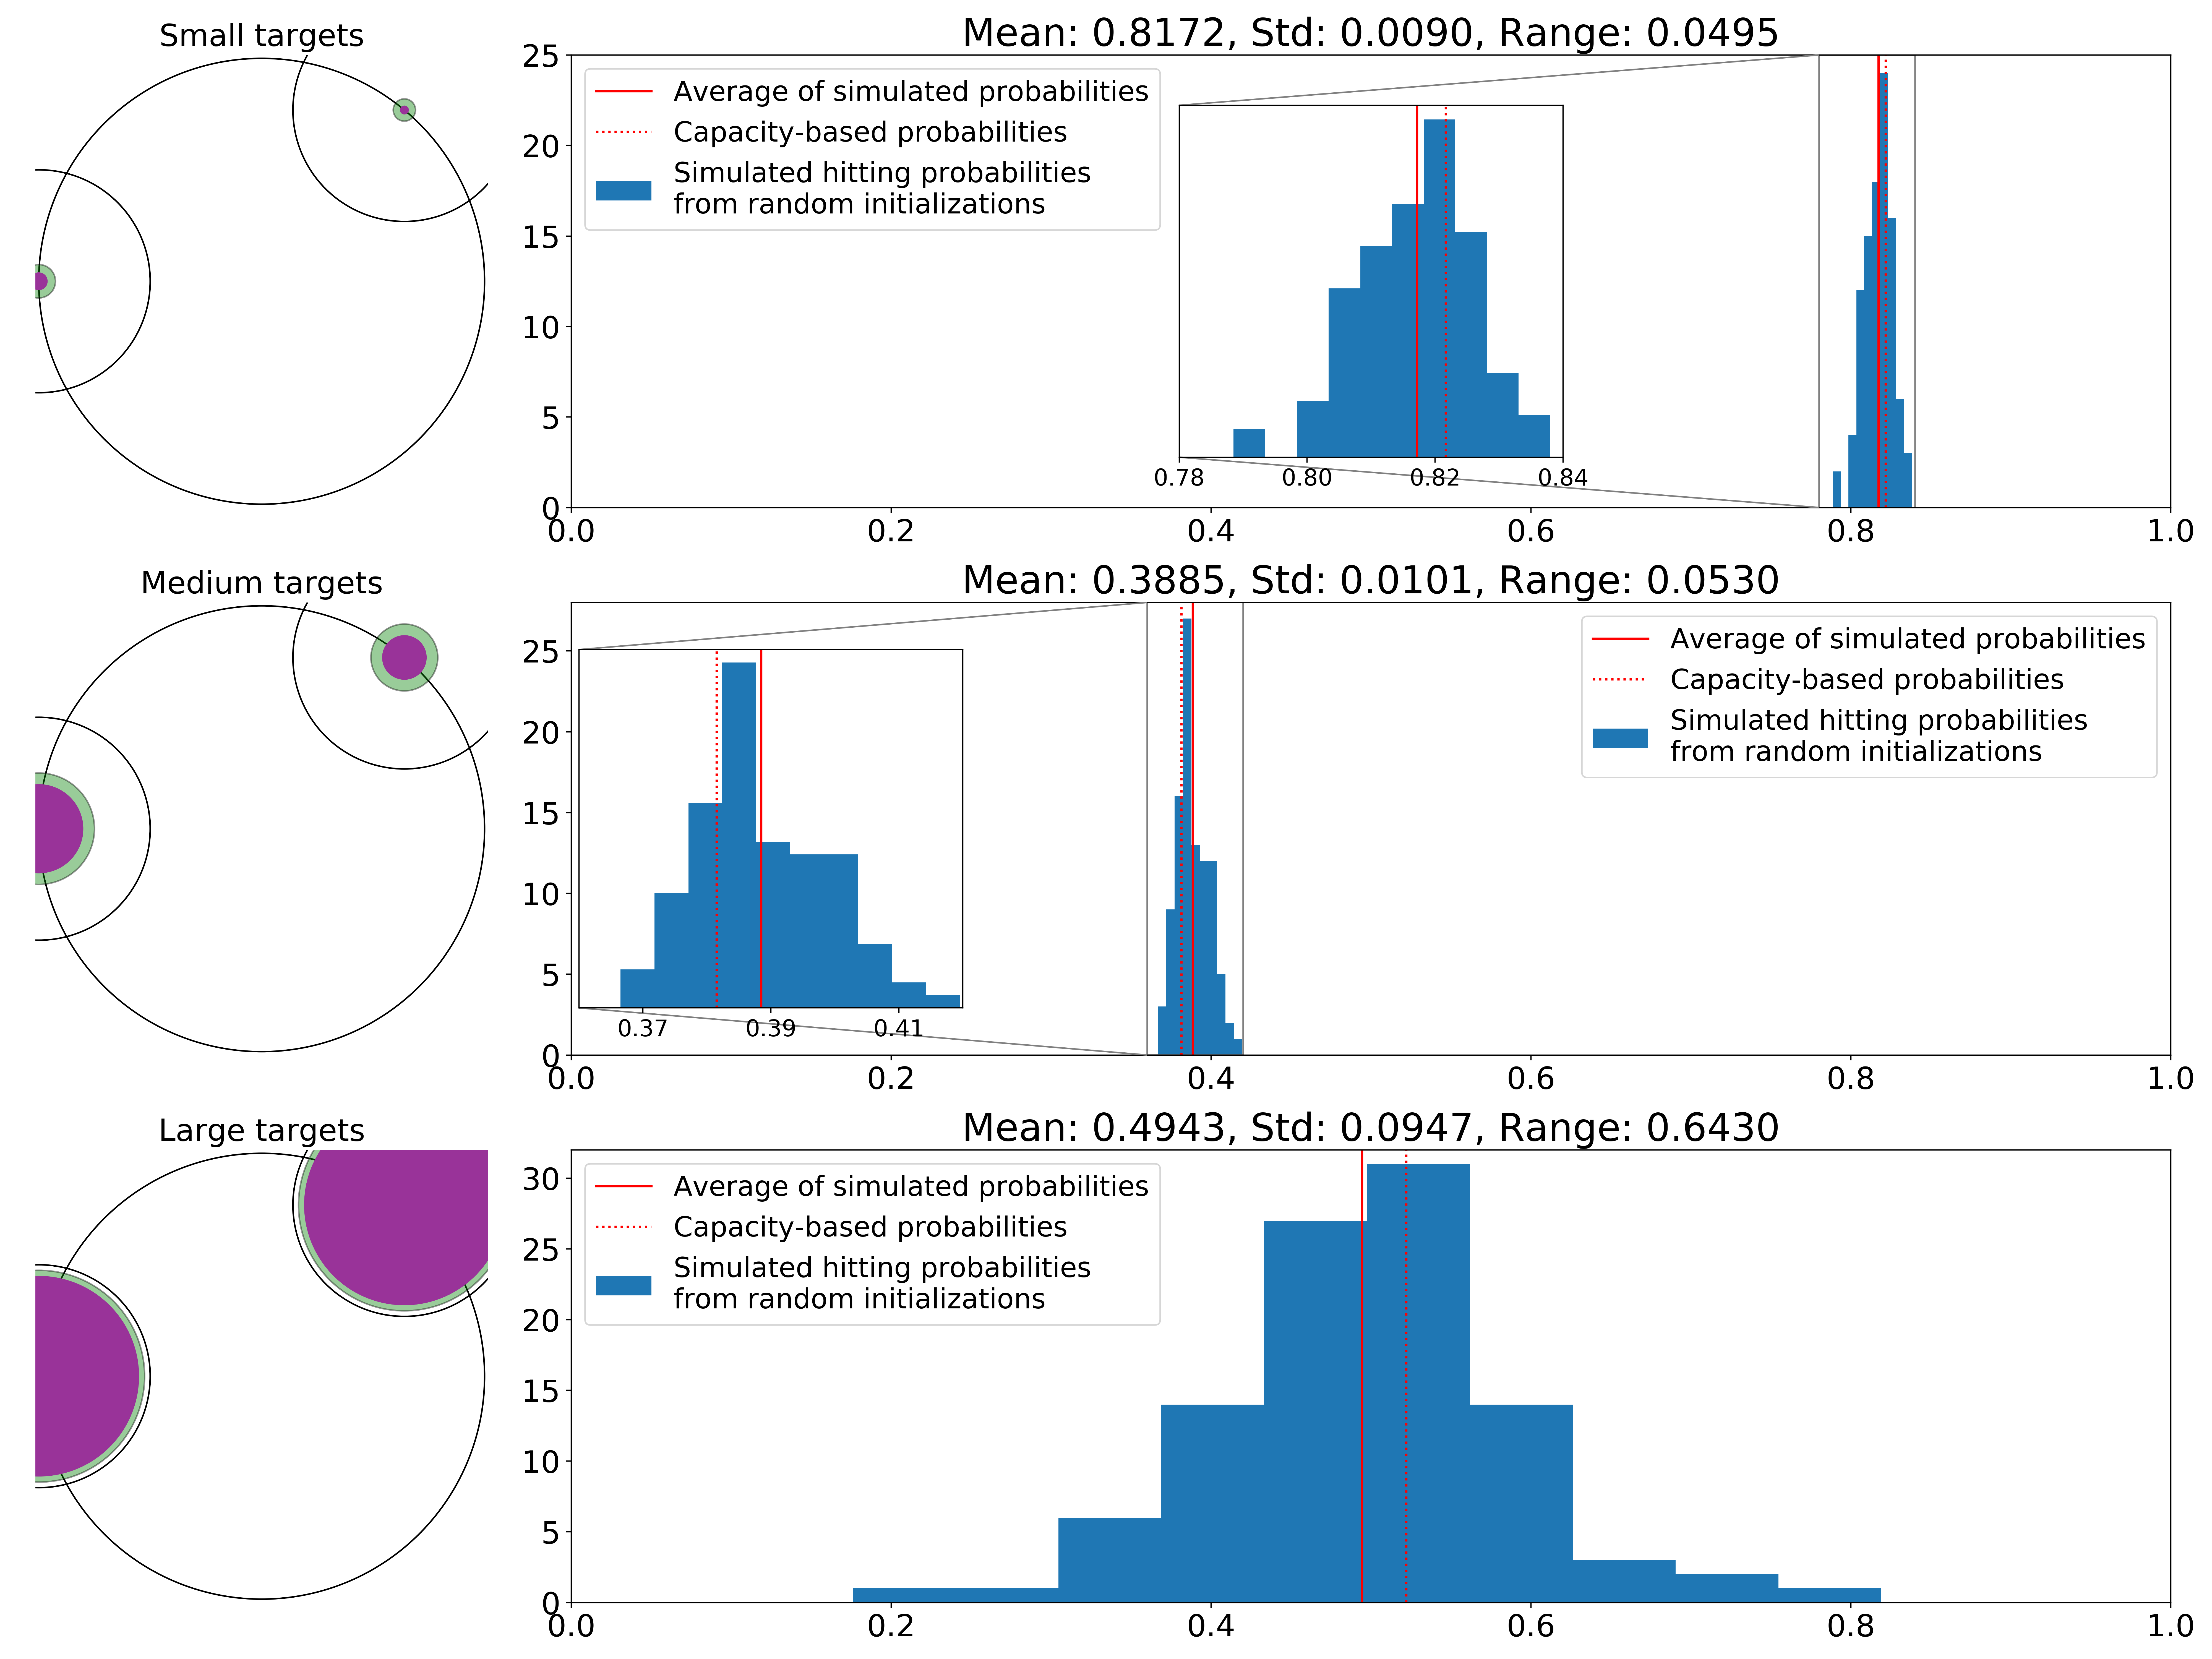
\includegraphics[width=\textwidth]{results_nontrivial.png}
    \caption{\label{fig:results_nontrivial} {\bf  Capacities and first-passage probabilities: nontrivial energy landscapes.} See Figure \ref{fig:results_brownian_motion}. The setup here is the same
 except that the targets $A$ and $B$ are only partially contained in $\Omega$, and the energy landscapes become complicated near the targets. 
The histograms show that the first-passage probabilities 
are largely independent of starting location for the small and medium targets, as they were in the previous set of experiments. 
In contrast, the first-passage probabilities for the large targets depend strongly on starting location. This is expected, since these targets are substantially larger than the corresponding targets from the previous experiments. (The size difference is 
even bigger than it might appear, given that these figures represent two-dimensional slices of a five-dimensional region.) 
In contrast to the Brownian motion examples, the complex landscape in these examples precludes an exact evaluation of 
$p_A$ (equation \ref{eqn:p_A}). Hence the dotted red line
represents the {\em estimated} value,
$\hat{p}_A$, computed using the shell method (cf. Figure 
\ref{fig:results_brownian_motion}). Nonetheless, 
these estimates fall within the span of the respective histograms in all three examples.}
\end{minipage}}
\end{figure}

\subsection{Nontrivial Landscape}\label{sec:nontrivial_results}
In the second set of experiments the targets $A$ and $B$ were only partially contained in $\Omega$, and the energy landscape $U$ was nontrivial.  We fixed the target centers at $x_A=(0.6402,0.7682,0.0,0,0,0.0)$ and  $x_B=(-1.0,0.0,0.0,0,0,0.0)$, and the outer radii at $r_\tA=r_\tB=0.5$.  We investigated three different cases with targets of different sizes: small (where $r_A=0.02, r_\dA=0.05, r_B=0.04$, and $r_\dB=0.075$), medium (where $r_A=0.1, r_\dA=0.15, r_B=0.2$, and $r_\dB=0.25$) and large (where $r_A=r_B=0.45$ and $r_\dA=r_\dB=0.475$). The  
specifications of the energy functions can be found in Appendix \ref{sec:energy_function}. Illustrations of the three set ups and corresponding results are shown in Figure \ref{fig:results_nontrivial}.  We will now revisit the three issues discussed in the previous examples, but in the context of the more complex landscapes surrounding the targets.

\subsubsection{Is the first-passage probability function 
 $\varepsilon$-flat?}
 \label{sec:nontrivial_flat}
 Following the same procedures used in \S\ref{sec:toy_constant}, we estimated $\varepsilon$-flatness 
from the spreads of the probability histograms: 
\begin{itemize}
    \item $\varepsilon\approx 0.0530$ when the targets are small
    \item $\varepsilon\approx 0.0495$ when the targets are medium
    \item $\varepsilon> 0.75$ when the targets are large
\end{itemize}
In the third example,
the first-passage probability function $h_{A,B}(x)$ can hardly be called flat.
Evidently, the large targets are not subject to the asymptotic guarantees offered in Theorem \ref{thm:epsilon_flat}.
In this circumstance, Theorem \ref{thm:main_thm} is irrelevant, and therefore we will discuss the remaining questions only in the context of the small and medium targets.


\subsubsection{How tight are the bounds in Theorem
\ref{thm:main_thm}?}
\label{sec:nontrivial_bounds}
In other words, how large is $\sup_x|h_{A,B}(x)-p_A|$ on $\Omega \setminus \tA \cup \tB$ compared to 
$\theepsrate$?
For Brownian motion (\S\ref{sec:B_D}), 
the capacities were derivable analytically (equation \ref{eqn:analytic_capacities}), which led to 
a closed-form expression for $p_A$. Here,
we followed the same reasoning as in 
\S\ref{sec:toy_capacity}
to get an approximation of the tightness of the theorem's bound, but replaced $p_A$ by  $\hat{p}_A$, the estimate computed from the shell method. The resulting value of $\hat{p}_A$, for each target size, is displayed in 
Figure \ref{fig:results_nontrivial}
as a dotted red line superimposed on the target-probability histogram. For both the small and medium targets, the estimated hitting probability lies within the range of the one-hundred sampled probabilities, as it did in the case of Brownian motion. 
Reasoning as we did there, these observations suggest that the true error may be better approximated by $\varepsilon$ rather than 
the $\theepsrate$
 guarantee given in the theorem. Specifically, the magnitudes of the ranges, 0.0530 and 0.0495 respectively, serve as ballpark upper bounds on the estimation errors for the first-passage probabilities for the small and medium targets.


\subsubsection{Is the shell method accurate and computationally efficient?}
How accurate is the shell method in these cases?  
In the absence of a closed-form expression for the capacities, we are forced to rely on an indirect measure.
In \S\ref{sec:nontrivial_bounds}, we used the shell method to estimate capacities and used those capacities to get hitting-probability estimates. These were in good agreement with
the results obtained from 200,000 runs of simulated diffusions
 (2,000 from each of 100 random starting points).
This, then, constitutes indirect evidence for the accuracy of the shell method, but with the important proviso that the estimated hitting probabilities only depend on the {\em ratio} of the (estimated) capacities, and not on the capacities themselves. 

To assess computational efficiency, we repeated the approach used for Brownian motion, step-by-step as laid out in \S\ref{sec:toy_shell}.
As noted there, one simulation run is nearly the same as using the shell method to estimate $p_A$, in terms of computational cost. 
Therefore, efficiency comparisons between the shell method (capacity-based) approach
and direct simulation come down to computing the number of simulation runs required to achieve comparable accuracy in estimating first-passage probabilities. In \S\ref{sec:toy_shell} we explored two interpretations of accuracy, which we repeat here, but using instead the results reported in Figure \ref{fig:results_nontrivial}:
\begin{enumerate}
\item 
For each target size (small and medium) and corresponding value
of $\hat{p}_A$, we used the probability histogram to estimate  $\mathbb{E}[| h_{A,B}(X) - \hat{p}_A |]$, the mean absolute error of the capacity-based method. The resulting accuracy measures came to 0.0078 for the small targets and 0.0095 for the medium targets. Then, using the respective probabilities of 0.8217 and 0.3893 (solid red lines), we conclude that in each case about 10,000 simulation runs would be needed to achieve an accuracy comparable to capacity-based approach. {\em In this sense, the capacity approach, based on shell-method estimates, is about 10,000 fold more efficient than direct simulation.}
\item
In the second interpretation, we consider the problem of estimating the mean first-passage probability for a randomly chosen starting position (approximately 0.8154 for the small targets and 0.3893 for the medium targets, based on 200,000 independent random samples). Errors in the capacity-based approach were about 0.0072 and 0.0089, which come from the differences in the positions of the red and dotted-red lines, but inflated to account for 
the expected sampling error when using a sample of size $n$=200,000.
Comparable accuracies would require about 12,000 simulation runs, for each of the small and medium targets. {\em Hence, from this point of view,  we would estimate that the capacity-based approach is about 12,000 fold more efficient than direct simulation.}
\end{enumerate}





%  ____ ___ ____   ____ _   _ ____ ____ ___ ___  _   _
% |  _ \_ _/ ___| / ___| | | / ___/ ___|_ _/ _ \| \ | |
% | | | | |\___ \| |   | | | \___ \___ \| | | | |  \| |
% | |_| | | ___) | |___| |_| |___) |__) | | |_| | |\  |
% |____/___|____/ \____|\___/|____/____/___\___/|_| \_|



\section{Summary and Discussion}
\label{sec:Discussion}

If a first-passage probability is nearly the same for every initial condition in a region $M$, then it can be well-approximated in terms of certain integrals.   We dub these integrals the ``first-passage capacities.''  These capacities can be approximately computed using a milestoning-like technique, as described in \S\ref{sec:Estimation}.  In Theorem \ref{thm:main_thm} we show that the error introduced by this approximation is small whenever hitting probabilities are sufficiently similar across different initial conditions inside a large region, $M$.  When this condition holds, we say that the hitting probabilities are ``$\varepsilon$-flat,'' where the coefficient $\varepsilon$ bounds  how much the hitting probabilities vary over the initial conditions.  Under what circumstances are hitting probabilities similar for all initial conditions in a large region, $M$?  Theorem \ref{thm:epsilon_flat} provides some sufficient conditions, though 
the concept is more general and we would expect some form
of $\varepsilon$-flatness to hold anytime the mixing rate of the diffusion is fast relative to the typical escape time from $M$.

The capacity of a given target is local, in the sense that the capacity integral is over a region in the neighborhood of the target. We have devised a Monte Carlo approach to estimating capacities that we call the shell method (\S\ref{sec:Estimation}).
In \S\ref{sec:Experiments} we provide evidence for the accuracy and computational efficiency of using estimated capacities and Theorem \ref{thm:main_thm} to compute 
first-passage probabilities. 
In a series of computational experiments we compared our capacity-based approach to the direct estimation of hitting probabilities using repeated runs of the diffusion. In each of these experiments, repeated simulation required at least three
orders-of-magnitude more computation to achieve comparable accuracy.

We were motivated by the narrow-escape problem, and in particular the potential connection to modeling the folding of large molecules. To the extent that folding can be thought of as a series of discrete steps, each requiring a rate-limiting search for  new connections in a large conformational space 
\cite{McLeish2005-dq,Goldberg1999-mv,Jacob1999-bs,Plaxco1998-iv,Wales2006-ur},
it might be possible to sidestep the exploratory phases by computing first-passage probabilities---one for each potential connection. An example might be the sequence of stem formations in the folding of structural RNA molecules.
The idea would be to model the creation of each new stem as the outcome of a first-passage problem, defined by the already established stems. Not only does the search, as opposed to the stem creation, have to be the rate-limiting step, but it must be slow enough to allow for the hitting probabilities to be nearly independent of the starting configuration. 
But the larger problem would be the possibility of the dissolution of an existing stem. RNA folding is not necessarily monotonic; stems come and go. Which will come first, the undoing of an existing stem or the creation of a new one?
Unless the undoing of a stem could be formulated as itself a target
or some kind of narrow escape, we would be forced to confront
the problem of estimating first-passage {\em times} in addition to probabilities. 

In general, it may turn out that estimating first-passage times is profoundly more difficult than estimating first-passage probabilities.  In this work we showed that the first-passage probabilities are sometimes invariant to the diffusion dynamics on the interior of a large set $M$, but the first-passing times will admit no such invariance.   If the dynamics inside of $M$ are genuinely intricate, it appears that estimating hitting times will always require a correspondingly intricate analysis.


\newpage
\appendix
\noindent {\bf APPENDIX}


%     _    ____  ____  _____ _   _ ____ _____  __     _
%    / \  |  _ \|  _ \| ____| \ | |  _ \_ _\ \/ /    / \
%   / _ \ | |_) | |_) |  _| |  \| | | | | | \  /    / _ \
%  / ___ \|  __/|  __/| |___| |\  | |_| | | /  \   / ___ \
% /_/   \_\_|   |_|   |_____|_| \_|____/___/_/\_\ /_/   \_\

\section{Three Perspectives on Hitting Probabilities}
\label{sec:three_perspectives}

Many of our results are based on the fact that hitting probabilities can actually be seen from three distinct perspectives.  To prepare for these results, we take a moment to review these three perspectives here.  Let $A,B\subset \Omega$, disjoint, open with smooth boundary.

\begin{enumerate}
\item Hitting probabilities.  Let $\tau_S \triangleq \inf\{t:\ X_t \in S\}$ for any set $S$ and $h_{A,B}(x) \triangleq \mathbb{P}(X_{\tau_{A\cup B}}\in \partial A|X_0=x)$.

\item Elliptic equation.  Let $h^\mathrm{dir}_{A,B}(x)$ denote the solution to the partial differential equation:
	    \begin{align}\label{eq:pde}
    0 &= \sum_{i = 1}^n b_i (x) \frac{\partial u
        (x)}{\partial x_i} + \frac{1}{2} \sum_{i = 1}^n \sum_{j = 1}^n a_{ij} (x)
        \frac{\partial^2 u (x)}{\partial x_i \partial x_j}\quad x\notin \bar A,\bar B\\
    1 &= u(x),x\in  A \nonumber \\
    0 &= u(x),x\in  B \nonumber \\
    0 &= \normal(x)^Ta(x)\nabla u(x), x \in \partial{\Omega}
    \nonumber
    \end{align}
This solution is unique and smooth.\cite{lieberman1986mixed}  What's more, it is equal to the hitting probability function: $h^\mathrm{dir}_{A,B}(x)=h_{A,B}(x)$ (cf.\ Section 6.7 of Chen\cite{chen2012symmetric}).
\item Variational form.  For any open set $S\subset \Omega$ let $\mathscr{E}_{S}(f,g)\triangleq \int_S \nabla f(x)^T a(x) \nabla g(x) \rho(dx)$ denote the ``Dirichlet Form'' of $f,g$ on the domain $S$.  Let $\mathscr L^2(S,\rho)$ denote the Hilbert space of functions on $S$ which are square-integrable with respect to $\rho$.  Let $\mathcal{H}^1(S,\rho)=W^{1,2}(S) \subset \mathscr{L}^2(S)$ denote the corresponding once-weakly-differentiable Hilbert Sobolev space.  We define $h^\mathrm{var}_{A,B}(x)$ as the solution to
    \begin{align*}
    \min_{u \in \mathcal H^1(S)} \quad & \mathscr{E}_S(u,u) \\
    \mbox{subject to} \quad & u(x)=1,x\in \partial A \\
     & u(x)=0,x\in \partial B
    \end{align*}
    where $S=\Omega \backslash (A\cup B)$.  This solution is unique and equal to $h^\mathrm{dir}_{A,B}$ on $S$ (cf.\ Section 4 of Dret\cite{dret2016partial}).
This variational perspective leads us to the notion of the ``condenser capacity'' associated with $h_{A,B}$.  It is defined as
    \[
    \capac{A}{\Omega \backslash B} \triangleq \mathscr{E}_S(h_{A,B},h_{A,B})
    \]
    where again $S=\Omega \backslash (A\cup B)=(\Omega \backslash B) \backslash A$.
\end{enumerate}
We will use all three of these perspectives to show our results.  For example, consider how the hitting probability perspective helps us show a result about capacities:
\begin{proposition}\label{prop:capacity}
Let $A\subset \tilde A,B\subset \tilde B$ with $\tilde A,\tilde B$ disjoint.  Then
\[
\capac{A\cup B}{\tilde A \cup \tilde B}=\capac{A}{\tilde A}+\capac{B}{\tilde B}
\]
\end{proposition}
\begin{proof}
This result is certainly known, but we include a proof here because we were unable to find a proof in the literature.  Since $\tilde A,\tilde B$ are disjoint and $X$ is continuous, the process cannot cross from one to the other without hitting the boundary.  Thus we have $\tau_{\partial \tilde A\cup \partial \tilde B \cup \partial A \cup \partial B}=\tau_{\partial \tilde A \cup \partial A}$ as long as $X_0\in\tilde A$.  We get a symmetric result if $X_0\in \tilde B$.  It follows that
\[
h_{A\cup B,(\tilde A\cup\tilde B)^c}(x) =
    \begin{cases}
    h_{A,\tilde A^c}(x) & \mbox{if }x\in \tilde A\\
    h_{B,\tilde B^c}(x) & \mbox{if }x\in \tilde B\\
    \end{cases}
\]
We can now use this probabilistic perspective to help us understand the capacity by articulating it as the Dirichlet form on the relevant hitting probability functions
\begin{align*}
\capac{A\cup B}{\tilde A \cup \tilde B}
        &= \int_{\tilde A\cup \tilde B \backslash (A\cup B)} \Vert \sigma \nabla h_{A\cup B,(\tilde A \cup \tilde B)^c}\Vert^2\rho(dx) \\
        &= \int_{\tilde A \backslash A} \Vert \sigma \nabla h_{A,\tilde A^c}\Vert^2\rho(dx)
            +\int_{\tilde B \backslash B} \Vert \sigma \nabla h_{B,\tilde B^c}\Vert^2 \rho(dx) \\
        &= \capac{A}{\tilde A}+\capac{B}{\tilde B}
\end{align*}
as desired.
\end{proof}

%     _    ____  ____  _____ _   _ ____ _____  __  ____
%    / \  |  _ \|  _ \| ____| \ | |  _ \_ _\ \/ / | __ )
%   / _ \ | |_) | |_) |  _| |  \| | | | | | \  /  |  _ \
%  / ___ \|  __/|  __/| |___| |\  | |_| | | /  \  | |_) |
% /_/   \_\_|   |_|   |_____|_| \_|____/___/_/\_\ |____/




\section{Proof of Theorem \ref{thm:epsilon_flat}}
\label{sec:proof_epsilon_flat}

\begingroup
\def\thetheorem{\ref{thm:epsilon_flat}}
\begin{theorem}
(Examples of $\varepsilon$-flatness).   Let $\bb{x,r} = \{y:\ \Vert x-y \Vert < r\}$ denote the ball of radius $r$ centered at $x$.  Recall that the process $X$ behaves according to the stochastic differential equation $dX_t = b(X_t)dt + \omega(X_t)dW_t$ contrained to lie inside a set $\Omega$ by normally reflecting boundaries.
\begin{enumerate}
    \item Let $\Omega \in \mathbb{R}^n, n\geq 3$ be convex and open with diameter less than or equal to 1.  Fix any points $x_A,x_B \in \mathbb{R}^n$.  For any $r,\varepsilon>0$ we can find $r'>0$ such that $h_{A,B}$ is $\varepsilon$-flat on $\Omega \backslash \bb{x_A,r}\cup \bb{x_B,r}$ for any $A\subset \bb{x_A,r'},B\subset \bb{x_A,r'}$ as long as $b(x)=0,\Omega(x)=I$ for $x \in \Omega \backslash \bb{x_A,r'}\cup\bb{x_B,r'}$.

    \item Fix $r,\varepsilon>0$ and also fix $r'<r$.  We can then find $n$ with the following property.  For any convex open set $\Omega \in \mathbb{R}^n$ with diameter less than or equal to 1, any $x_A,x_B$ such that $\bb{x_A, r},\bb{x_B, r} \subset \Omega$, and any $A\subset \bb{x_A, r'}, B \subset \bb{x_B, r'}$, we have that $h_{A,B}$ is $\varepsilon$-flat on $\Omega \backslash \bb{x_A, r} \cup \bb{x_B, r}$ as long as $b(x)=0,\Omega(x)=I$ for $x \in \Omega \backslash \bb{x_A,r'}\cup\bb{x_B,r'}$.
\end{enumerate}
\end{theorem}
\addtocounter{theorem}{-1}
\endgroup

\begin{proof}
Let $\dot A=\bb{x_A,r'},\dot B=\bb{x_B,r'}$.  Let $\{Z_t\}_t$ denote a Brownian motion trapped inside $\Omega$ and coupled to $X$ such that $X_{t}=Z_{t}$ for all $t\leq\tau=\left\{ \inf t:\ X_{t}\in\dot{A}\cup\dot{B}\right\} $ (we can do this because we assumed that $X$ behaves like Brownian motion outside of $\dot{A},\dot{B}$).  Let $Z_\infty$ denote the stationary distribution of $Z$, i.e. the uniform distribution on $\Omega$.
Using Lemma \ref{lem:uniform_ergodicity}, we have that
\[
\left|\mathbb{E}\left[h_{A,B}(Z_{t})-h_{A,B}(Z_{\infty}) | Z_0 =x \right]\right|\leq\frac{1}{t} \qquad \forall x
\]
On the other hand, Dynkin's formula gives that
\[
h_{A,B}(x)=\mathbb{E}\left[h_{A,B}(Z_{\tau\wedge t}) | Z_0=x\right]\qquad\forall t,x
\]
Putting those two facts together:
\begin{align*}
& \left|h_{A,B}(x)-\mathbb{E}\left[h_{A,B}(Z_{\infty})\right]\right| \\
=& \left|\mathbb{E}\left[h_{A,B}(Z_{\tau\wedge t})  - h_{A,B}(Z_{\infty}) | Z_0=x\right]\right|\\
 \leq & \left|\mathbb{E}\left[h_{A,B}(Z_{\tau\wedge t}) - h_{A,B}(Z_{t}) |Z_0=x\right]\right|+\left|\mathbb{E}\left[h_{A,B}(Z_{t}) -h_{A,B}(Z_{\infty}) | Z_0=x\right]\right|\\
 \leq& \mathbb{P}\left(\tau\leq t |Z_0 = x\right)+\frac{1}{t}
\end{align*}
To make this small, it thus suffices to get $t$ large but keep $\mathbb{P}\left(\tau\leq t\right)$ small.  In short, it suffices to show that $\tau$ is usually big.  We prove this differently in the two different cases:

\begin{enumerate}
    \item The first example follows because the targets are vanishing into nothing, so it is no surprise that the time to hit the targets will get longer and longer.  However, note that this intuition is valid only because  the ambient dimension $n$ is at least three (which we have assumed throughout).  A formal proof of this argument can be found in Lemma \ref{lem:longtime_diamater}.

    \item The second example is similar; even though the targets maintain the same diameter, their relative volume is vanishing because the ambient dimension $n$ is increasing.  Thus the targets are effectively becoming smaller, so the hitting time increases.  This matter is a bit trickier, and so for this second case note we have made additional requirements that $\bb{x_A,r},\bb{x_B,r} \subset \Omega$.  A formal proof of this argument can be found in Lemma \ref{lem:longtime}.
\end{enumerate}

\end{proof}

%%%%%%%%%%%%%%%%%%%%%%
%%%%%%%%%%%%%%%%%%%%%%

\begin{lemma}
\label{lem:uniform_ergodicity}(Uniform ergodicity) Let $\Omega\subset\mathbbm{R}^d$ be a convex set with diameter $\xi$ and let $M$ denote a Brownian motion trapped by reflecting boundaries inside $\Omega$.  The distribution of $M_t$ converges uniformly to the uniform distribution, in the sense that:
%
\[
\sup_{f:\ \Omega\rightarrow [0,1]} | \mathbb{E}[f(M_t) - f(Z)|M_0=x]| \leq \xi^2/4t \qquad \forall x\in \Omega, t>0
\]
%
where $Z$ is uniformly distributed on $\Omega$.
\end{lemma}
\begin{proof}
Per Loper \cite{Loper2018},
\[
\sup_{f:\ \Omega\rightarrow [0,1]} | \mathbb{E}[f(M_t) - f(Z)|M_0=x]| \leq \mathbbm{P}(\tau>4t)
\]
where $\tau$ is the first exit time of a one-dimensional Brownian motion from the interval $[-\xi,\xi]$ when initialized at the origin. Dynkin's formula gives that $\mathbb{E}[\tau]=\xi^2$. Hence, by the Markov inequality, $\mathbbm{P}(\tau>4t)\leq \xi^2/4t$.
\end{proof}

%%%%%%%%%%%%%%

\begin{lemma}
\label{lem:longtime_diamater}
Let Z denote a Brownian motion trapped inside a convex bounded open set $\Omega\subset\mathbb{R}^{n}$ with smooth boundary.  We further assume that $n\geq3$. Fix $x\in\mathbb{R}^{n}$ and $r,\epsilon>0$. Let $\tau_{A}$ denote $\inf\{t:\ Z_{t}\in A\}$ for any set A. We can always find $r_1>0$ such that $\mathbb{P}(\tau_{A}<1/\epsilon|Z_{0}=z)<\epsilon$ for all $z\notin\bb{x,r_3}$ and all $A\subset\bb{x,r_1}$.
\end{lemma}
\begin{proof}
First consider the case that $x \in \Omega$.  To measure the time it takes to hit $\bb{x,r_1}$, we will make use of two additional concentric spheres around $x$.  First, find $r_3$ such that $\bb{x,r_3} \subset \Omega$.  Second, let $r_2 =\sqrt{r_1 r_3}$, an intermediate radius.    We will use these spheres to break the trajectory of $Z$ into smaller manageable pieces. If $\left\Vert Z_{0}-x\right\Vert >r_3$,
the first part of the trajectory must carry it to a radius of $r_2$ before it reaches $r_1$.
The next part of the trajectory will then do one of two things: either
it will carry on to $r_1$ or it will first exit the ball of radius
$r_3$. Assuming it exits the ball of radius $r_3$, the strong Markov
property can be used to show that we are essentially in the same place
we started. Under this latter condition, the total time will be the
the time we've spent so far plus a new variable which has the same
properties as the original time. We can use this recursive relation to put a lower
bound on the overall time.

Let us make this rigorous. To measure the tails of $\tau$, we will
be interested in
\[
g(z)=\mathbb{E}\left[e^{-\frac{1}{2}\tau}|Z_{0}=z\right]
\]
To get a lower bound on the moments of $\tau$, we need to get an upper bound on this object.  To do so, we will use two objects of interest:
\begin{align*}
g_3 & =\sup_{z:\ \left\Vert z-x\right\Vert =r_3}g(z)\\
g_2 & =\sup_{z:\ \left\Vert z-x\right\Vert =r_2}g(z)
\end{align*}
using two stopping times of interest:
\begin{align*}
T_{2} & =\inf\{t:\ \Vert Z_{t}-x\Vert=r_2\}\\
T_{3} & =\inf\{t>T_{1}:\ \Vert Z_{t}-x\Vert=r_3\}
\end{align*}
Applying the strong Markov property, we observe that
\begin{align*}
g_{2} & =\sup_{z:\ \left\Vert z-x\right\Vert =r_2}\mathbb{E}\left[\mathbb{E}\left[e^{-\frac{1}{2}\tau}|Z_{T_{3}\wedge\tau}\right]|Z_{0}=z\right]\\
 & =\sup_{z:\ \left\Vert z-x\right\Vert =r_2}\mathbb{E}\left[e^{-\frac{1}{2}T_{3}\wedge\tau}g(Z_{T_{3}\wedge\tau})|Z_{0}=z\right]\\
 & \leq\sup_{z:\ \left\Vert z-x\right\Vert =r_2}\mathbb{E}\left[e^{-\frac{1}{2}T_{3}}g_{3}\mathbb{I}_{T_{3}<\tau}+e^{-\frac{1}{2}\tau}\mathbb{I}_{T_{3}>\tau}|Z_{0}=z\right]
\end{align*}
On the other hand, applying the continuity of Brownian motion we have
that $T_{2}<\tau$ whenever $Z_0$ lies outside the ball of radius $r_2$, so
\[
g_3=\sup_{z:\ \left\Vert z-x\right\Vert =r_3}\mathbb{E}\left[e^{-\frac{1}{2}T_{2}}g(T_{2})|Z_{0}=z\right]\leq g_2
\]
So in fact
\begin{align*}
g_3 & \leq\sup_{z:\ \left\Vert z-x\right\Vert =r_2}\mathbb{E}\left[e^{-\frac{1}{2}T_{3}}\mathbb{I}_{T_{3}<\tau}g_3+e^{-\frac{1}{2}\tau}\mathbb{I}_{T_{3}>\tau}|Z_{0}=z\right]\\
g_3 & \leq\frac{\sup_{z:\ \left\Vert z-x\right\Vert =r_2}\mathbb{E}\left[e^{-\frac{1}{2}\tau}\mathbb{I}_{T_{3}>\tau}|Z_{0}=z\right]}{1-\sup_{z:\ \left\Vert z-x\right\Vert =r_2}\mathbb{E}\left[e^{-\frac{1}{2}T_{3}}\mathbb{I}_{T_{3}<\tau}|Z_{0}=z\right]} = L
\end{align*}

To calculate this upper-bound $L$, defined above, Wendel gives explicit formulas (cf.\ \cite{Wendel1980-sj}).  We caution that in this document a somewhat nonstandard notation is used, namely Wendel uses $\mathbb{E}[A;B]$ to indicate $\mathbb{E}[A\times\mathbb{I}_B]$.  For any $z$ with $\Vert z-x\Vert=r_2$, Wendel uses the symmetry of the problem to show that
%
\begin{align*}
\mathbb{E}\left[e^{-\frac{1}{2}\tau}\mathbb{I}_{T_{3}>\tau}|Z_{0}=z\right]&=\left(\frac{r_{1}}{r_{2}}\right)^{h}\frac{I(r_{3})K(r_{2})-I(r_{2})K(r_{3})}{I(r_{3})K(r_{1})-I(r_{1})K(r_{3})}\\
\mathbb{E}\left[e^{-\frac{1}{2}\tau}\mathbb{I}_{T_{3}<\tau}|Z_{0}=z\right]&=\left(\frac{r_{3}}{r_{2}}\right)^{h}\frac{I(r_{1})K(r_{2})-I(r_{2})K(r_{1})}{I(r_{1})K(r_{3})-I(r_{3})K(r_{1})}
\end{align*}
%
where $h=(n-2)/2$ and $I,K$ denote the modified Bessel functions of order $h$.  This leads to the following explicit formula for $L$.
\begin{gather}
L=\frac{\left(\frac{r_{1}}{r_{2}}\right)^{h}\left(I_{3}K_{2}-I_{2}K_{3}\right)}{I_{2}K_{1}\left(\frac{I_{3}}{I_{2}}-\left(\frac{r_{3}}{r_{2}}\right)^{h}\right)+I_{1}K_{2}\left(\left(\frac{r_{3}}{r_{2}}\right)^{h}-\frac{K_{3}}{K_{2}}\right)}
\label{eq:Lforlongtime}
\end{gather}
where we denote $I_1=I(r_1),K_1=K(r_1),I_2=I(r_2)$, and so-on.  To prove our result, it thus suffices to show we can drive $L$ to zero by taking $n$ sufficiently large.

The numerator of $L$ in Equation (\ref{eq:Lforlongtime}) converges to zero as $r_1\rightarrow 0$, because $\frac{r_1}{r_2}\rightarrow 0,h>0$ and the other terms are constant.  On the other hand, the denominator explodes, because as $r_1\rightarrow0$ we have
\begin{align*}
\left(\frac{I_{3}}{I_{2}}-\left(\frac{r_{3}}{r_{2}}\right)^{h}\right)K_{1}I_{2}\rightarrow+\infty\\
\left(\left(\frac{r_{3}}{r_{1}}\right)^{h}-\frac{K_{3}}{K_{2}}\right)I_{1}K_{2}\rightarrow0
\end{align*}
These limits follow immediately from three properties of Bessel functions:
\begin{itemize}
    \item $K(x)\rightarrow \infty,I(x)\rightarrow 0$ as $x\rightarrow 0$ for $h>0$
    \item $K(x),I(x)>0$ for $x>0,h>0$
    \item $\frac{I(y)}{I(x)} > \left(\frac{y}{x}\right)^{h}$ for $y>x$ and $h>0$
\end{itemize}
The first two properties are well-known and can be found in DLMF (cf. \cite{noauthor_undated-ti}); the second can be found in Baricz (cf. \cite{noauthor_undated-ti,baricz2010bounds}). In conclusion, since the numerator vanishes and the denominator explodes, we have that overall $L$ vanishes.  Applying a Chernoff bound, we have our result for the case that $x \in \Omega$.

What happens if $x$ is not in the closure of $\Omega$?  Then by taking $r_1$ sufficiently small we can ensure that $A \cap \Omega = \emptyset$, so $\tau = \infty$.  Thus the result is proved automatically.

What if $x$ is precisely on the boundary of $\Omega$?  Here we must use the smoothness of the boundary of $\Omega$.  By picking $r_3$ sufficiently small, the smoothness guarantees that $\Omega$ is arbitrarily well-approximated by a half-plane when restricted to a ball $\bb{x,r_3}$.  In this half-plane case, identical arguments to the ones above can be used to argue that we can always take a $r_1$ that is yet smaller than $r_3$ and ensure that the hitting time is arbitrarily long.  Finally, to account for the slight discrepancy between the half-plane case and the actual case for some finite $r_3$, we appeal to the continuity of the Poisson equation which governs $g$ with respect to boundary condition (cf. \cite{strang1972approximation}).
\end{proof}


%%%%%%%%%%%%%%

\begin{lemma}
\label{lem:longtime} Fix $0<\epsilon$ and $0<r_1<r_3$.  Then we can always find an $n$ with the following property.  Pick any open set $\Omega \in \mathbb{R}^n$, any $x$ satisfying $\bb{x,r_3}\subset \Omega$, and any $x_0 \notin \bb{x,r_3}$.  Consider a Brownian motion $Z$ trapped inside $\Omega$ by reflecting boundaries and let $\tau$ denote the first hitting time of the process to $\bb{x,r_1}$.  Our choice of $n$ guarantees that
\[
\mathbb{P}(\tau < 1/\epsilon|Z_t=x_0) \leq \epsilon
\]
\end{lemma}
\begin{proof}
Following the same arguments found in Lemma \ref{lem:longtime_diamater}, we again obtain that $\mathbb{E}[e^{-\tau/2}|Z_0=x_0]$ is bounded by
\begin{gather}
L=\frac{\left(\frac{r_{1}}{r_{2}}\right)^{h}\left(I_{3}K_{2}-I_{2}K_{3}\right)}{I_{2}K_{1}\left(\frac{I_{3}}{I_{2}}-\left(\frac{r_{3}}{r_{2}}\right)^{h}\right)+I_{1}K_{2}\left(\left(\frac{r_{3}}{r_{2}}\right)^{h}-\frac{K_{3}}{K_{2}}\right)}
\end{gather}
To show our proof, it thus suffices to show we can drive this quantity to zero and then apply a Chernoff bound.

Let us first look at the numerator of $L$ in Equation \ref{eq:Lforlongtime}.  Asymptotics from the DLMF give that as $h \rightarrow \infty$ we have
\begin{align*}
I(x) \sim \frac{x^h}{2^h\Gamma(h+1)} & & K(x) \sim \frac{2^h\Gamma(h+1)}{(2h)x^h}
\end{align*}
Here by $f_1(h)\sim f_2(h)$ we mean ``asymptotic equivalence,'' i.e.\ $\lim_{h\rightarrow\infty}f_1(h)/f_2(h)=1$.  Plugging these in, we see that both terms in the numerator are asymptotically vanishing.

Now let us turn to the denominator.  Using the asymptotic formula above, we first note that
\begin{align*}
\left(\frac{r_{3}}{r_{2}}\right)^{h}I_{1}K_{2}&\sim\frac{1}{2h}\left(\frac{r_{3}r_{1}}{r_{2}^{2}}\right)^{h}=\frac{1}{2h}\rightarrow0\\
-\frac{K_3}{K_{2}}I_{1}K_{2}&\sim-\frac{1}{2h}\left(\frac{r_{1}}{r_{3}}\right)^{h}\rightarrow0
\end{align*}
So those terms are negligible.  However, the other two terms of the denominator are in fact exploding: one to positive infinity and one to negative infinity.  To understand this delicate balance, we these we turn to Lemma \ref{lem:bessel}.  Applying this Lemma and the asymptotics of the DLMF, we obtain that
\begin{align*}\left(\frac{I_{3}}{I_{2}}-\left(\frac{r_{3}}{r_{2}}\right)^{h}\right)K_{1}I_{2}&\geq\frac{r_{3}^{h}}{\cancel{I_{2}}}\times\frac{r_{3}^{2}-r_{2}^{2}}{2^{h+2}\Gamma(h+2)}K_{1}\cancel{I_{2}}\\
&\sim r_{3}^{h}\times\frac{r_{3}^{2}-r_{2}^{2}}{2^{h+2}\Gamma(h+2)}\frac{2^{h}\Gamma(h+1)}{2hr_{1}^{h}}\\&=\left(\frac{r_{3}}{r_{1}}\right)^{h}\left(\frac{r_{3}^{2}-r_{2}^{2}}{8h(h+1)}\right)
\end{align*}
which is indeed exploding to positive infinity as $h=(n-2)/2 \rightarrow \infty$.

Thus, since the numerator vanishes and the denominator explodes to positive infinity, we have that $L$ vanishes as $n\rightarrow \infty$.
\end{proof}

\begin{lemma}\label{lem:bessel}
Let $I$ denote the modified bessel function of the first kind of order $h$.  If $a>b$ then
    \[
    \frac{I ( a)}{I (b)} - \left(\frac{a}{b} \right)^h
    \geq
    \frac{a^h}{I(b)}\times\frac{a^{2} -b^{2}}{2^{h+2}\Gamma(h+2)}
    \]
\end{lemma}
\begin{proof}
Recall that $I$ may be defined as
\[
I(x) = \sum_{m=0}^\infty \frac{x^{h+2m}}{2^{h+2m}\Gamma(m+h+1)\Gamma(m+1)}
\]
Thus
\begin{align*}
\frac{I ( a)}{I (b)} - \left(\frac{a}{b} \right)^h
    &= \frac{I(a)b^h-a^hI(b)}{b^hI(b)}  \\
    &= \frac{a^hb^h\sum_{m=0}^\infty \frac{a^{2m} -b^{2m}}{2^{h+2m}\Gamma(m+h+1)\Gamma(m+1)}}{b^{h}I(b)}
\end{align*}
Since $a>b$, we have that $a^{2m} -b^{2m}$ is always positive.  Thus we can get a lower bound by simply taking one of the terms.  Choosing $m=1$, we get our final result.
\end{proof}

%  ____ _____     _______ ____   ____ _____ _   _  ____ _____
% |  _ \_ _\ \   / / ____|  _ \ / ___| ____| \ | |/ ___| ____|
% | | | | | \ \ / /|  _| | |_) | |  _|  _| |  \| | |   |  _|
% | |_| | |  \ V / | |___|  _ <| |_| | |___| |\  | |___| |___
% |____/___|  \_/  |_____|_| \_\\____|_____|_| \_|\____|_____|



\section{Proof of Theorem \ref{thm:main_thm}}
\label{sec:proof_thm}

Let $A\subset\tilde A\subset\Omega,B\subset\tilde B\subset\Omega$.  Let $\tilde A,\tilde B$ be disjoint and
$h_{A,B}(x)$  $\varepsilon$-flat with respect to $\Omega \backslash (\tilde A \cup \tilde B)$. We assume the set boundaries are all smooth.

Under these conditions, we will show we can use local capacities to get good approximations for $h_{A,B}(x)$ when $x\notin \tilde A,\tilde B$.  To do so, our key idea is to uncover upper and lower bounds on the value of the Dirichlet form applied to this function, $\mathscr{E}(h_{A,B},h_{A,B})$.  We will see that these bounds can be understood in terms of local capacities, and the resulting inequalities will then yield our main result in the form of Theorem \ref{thm:main_thm}.

\begin{lemma}  Let $S=\Omega \backslash (A\cup B)$.  The Dirichlet form of $h_{A,B}$ on $S$ can be upper-bounded in terms of the capacities:
\[ \mathscr{E}_S(h_{A,B}, h_{A,B}) \leqslant \frac{\tmop{cap} (A, \tilde{A}) \tmop{cap} (B,
\tilde{B})}{\tmop{cap} (A, \tilde{A}) + \tmop{cap} (B, \tilde{B})} \]
\end{lemma}
\begin{proof}
We recall from Appendix \ref{sec:three_perspectives} that
%
\[
\mathscr{E}_S(h_{A,B}, h_{A,B}) = \capac{A}{\Omega \backslash B} \leq \mathscr{E}_S (u,u)
\]
%
for any $u$ with $u(\partial A) = 1,u(\partial B) = 0$.  Thus, to prove an upper bound it suffices to find any such function for which we can calculate $\mathscr{E}(u,u)$.  To this end, consider
%
\[
u_c (x) \triangleq \left\{ \begin{array}{ll}
(1 - c) h_{A, \widetilde{A}^c} (x) + c & \tmop{if} x \in \tilde{A} \\
c (1 - h_{B, \widetilde{B}^c} (x)) & \tmop{if} x \in \tilde{B} \\
c & \mbox{otherwise}
\end{array} \right.
\]
%
These functions are well-suited to giving us upper bounds on $\mathscr{E}_S (h_{A,B}, h_{A,B})$.  Indeed:
\begin{itemize}
\item $u_c(\partial A)=1,u_c(\partial B)=0$.  In fact, $u_c$ takes a constant value $c$ outside of $\tilde A,\tilde B$, drops smoothly in $\tilde B$ to achieve 0 on $\partial B$, and rises smoothly in $\tilde A$ to achieve 1 on $\partial \tilde A$.
\item Noting that $u_c$ is written as a piecewise combination of hitting probability functions, we see that its Dirichlet form can be calculated in terms of capacities on local regions: $\mathscr{E}_S(u_c,u_c) = (1 - c)^2 \tmop{cap} (A, \tilde{A}) + c^2 \tmop{cap} (B, \tilde{B})$.
\end{itemize}
Thus the $u_c$ functions give us a practical way to calculate upper bounds:
\[
\mathscr{E}_S(h_{A,B}, h_{A,B})\leq (1 - c)^2 \tmop{cap} (A, \tilde{A}) + c^2 \tmop{cap} (B, \tilde{B})
\]
This inequality holds for any value of $c$.  To get the best bound, we can take derivatives to minimize the right hand side with respect to $c$.  The result is
\[
c^* = \frac{\capac{A}{\tilde A}}{\capac{A}{\tilde A}+\capac{B}{\tilde B}}
\]
Plugging this into the previous equation, we obtain our final result.
\end{proof}

%%%%%%%%%%%
%%%%%%%%%%%

\begin{lemma}  Let $S=\Omega \backslash (A\cup B)$.  Let $m = \frac{1}{2} (\sup_{x \notin \tilde A,\tilde B} h_{A,B} (x) + \inf_{x \notin \tilde A,\tilde B} (h_{A,B} (x)))$.  The Dirichlet form of $h_{A,B}$ can be lower-bounded in terms of $m$ and the capacities:
\[\mathscr{E}_S (h_{A,B}, h_{A,B}) \geq
   \left( 1 - m - \frac{\varepsilon}{2} \right)^2 \tmop{cap} (A,\tilde{A}) \indicatorf{m\leq 1-\frac{\varepsilon}{2}} +
   \left( m- \frac{\varepsilon}{2} \right)^2 \tmop{cap} (B, \tilde{B})\indicatorf{m\geq \frac{\varepsilon}{2}}
\]
\end{lemma}
\begin{proof}
Recall that $\mathscr{E}_S(h_{A,B}, h_{A,B})$ can be expressed as an integral over $S$.  We decompose this into three integrals: one over $\tilde A$, one over $\Omega \backslash \tilde A,\tilde B$, and one over $\tilde B$.
\[
\mathscr{E}_S (h_{A,B}, h_{A,B}) = \int_{\tilde A \backslash A} \Vert \sigma \nabla h_{A,B}\Vert^2 \rho(dx)
                                 + \int_{\tilde B \backslash B} \Vert \sigma \nabla h_{A,B}\Vert^2 \rho(dx)
                                 + \int_{\Omega \backslash \tilde A,\tilde B} \Vert \sigma \nabla h_{A,B}\Vert^2 \rho(dx)
\]
Since the integrand is always positive, we can get a lower bound by simply ignoring the integral over $\Omega \backslash \tilde A,\tilde B$ and focusing on the integrals over $\tilde A,\tilde B$.  The $\tilde A,\tilde B$ integrals can be lower-bounded using capacities.

For example, let us focus on the $A$ integral.  There are two different possibilities we must consider:
\begin{itemize}
\item If $m>1-\varepsilon/2$ we will simply note that the integral over the $\tilde A$ region is non-negative.
\item If $m\leq 1-\varepsilon/2$, then we define
    \[
    u_A (x) \triangleq \frac{h_{A,B} (x) - m - \frac{\varepsilon}{2}}{1 - m - \frac{\varepsilon}{2}}
    \]
    Note that  $h_{A,B}(x)=1$ for $x \in \partial A$ and the $\varepsilon$-flatness condition shows that $h_{A,B}(x) \leq m + \frac {\varepsilon}{2}$ for $x \in \partial \tilde A$.  Thus $u_A(\partial A)\geq1,u_A(\partial \tilde A)\leq 0$.  Lemma \ref{lem:inequalityboundaryvar} from Appendix \ref{sec:inequalityboundaryvar} may then be applied to yield that $\mathscr{E}_{\tilde A \backslash A}(u_A,u_A) \geq \capac{A}{\tilde A}$.  We can thus obtain the bound
    \begin{align*}
    \int_{\tilde A \backslash A} \Vert \sigma \nabla h_{A,B}\Vert^2 \rho(dx)
	 &= \left(1 - m - \frac{\varepsilon}{2}\right)^2 \mathscr{E}_{\tilde{A} \backslash A}(u_A,u_A)\\
         &\geq \left(1 - m - \frac{\varepsilon}{2}\right)^2 \capac{A}{\tilde A}
    \end{align*}
\end{itemize}
Putting these two possibilities together, we obtain
\[
\int_{\tilde A \backslash A} \Vert \sigma \nabla h_{A,B}\Vert^2 \rho(dx) \geq \left(1 - m - \frac{\varepsilon}{2}\right)^2 \capac{A}{\tilde A}\indicatorf{m\leq 1-\frac{\varepsilon}{2}}
\]
Applying the same ideas to the integral over $\tilde B$, we obtain our result.
\end{proof}

%%%%%%%%%%%
%%%%%%%%%%%

We are now in a position to prove Theorem \ref{thm:main_thm} from the main text:

\begingroup
\def\thetheorem{\ref{thm:main_thm}}
\begin{theorem}
Assume that  $h_{A,B}(x)$ is $\varepsilon$-flat relative to
$\Omega \backslash (\tilde A \cup \tilde B)$.
Then the first-passage probabilities can be well-approximated in terms of the target capacities:
\[ \sup_{x \notin \tilde A,\tilde B} \left| h_{A,B} (x) - \frac{\capac{A}{\tilde A}}{\capac{A}{\tilde A}+\capac{B}{\tilde B}} \right| \leqslant \varepsilon + \sqrt{\varepsilon/2} \]
\end{theorem}
\addtocounter{theorem}{-1}
\endgroup


\begin{proof}

To simplify notation, let $\capA=\capac{A}{\tilde A}$ and $\capB=\capac{B}{\tilde B}$.  Applying the previous two lemmas together, we obtain the inequality
\[
\frac{\capA \capB}{\capA +\capB}
\geq \mathscr{E}(h_{A,B},h_{A,B}) \geq
\left( 1 - m - \frac{\varepsilon}{2} \right)^2 \capA \indicatorf{m\leq 1-\frac{\varepsilon}{2}} +
   \left( m- \frac{\varepsilon}{2} \right)^2 \capB \indicatorf{m\geq \frac{\varepsilon}{2}}
\]
where $m = \frac{1}{2} (\sup_{x \notin \tilde A,\tilde B} h_{A,B} (x) + \inf_{x \notin \tilde A,\tilde B} (h_{A,B} (x)))$.  In analyzing this inequality, there are three possibilities to consider.
\begin{itemize}
    \item If $m \in (\varepsilon/2,1-\varepsilon/2)$, the quadratic formula yields
    \begin{eqnarray*}
    m & \geqslant & \frac{\capA}{\capA + \capB} + \frac{
    \frac{\varepsilon}{2}(\capB - \capA) -
    \sqrt{\capA \capB \varepsilon( 2 - \varepsilon)}}{\capA+\capB}\\
    m & \leqslant & \frac{\capA}{\capA + \capB} + \frac{
    \frac{\varepsilon}{2}(\capB - \capA) +
    \sqrt{\capA \capB \varepsilon( 2 - \varepsilon)}}{\capA+\capB}
    \end{eqnarray*}
    Applying $\left|\frac{\capB - \capA}{\capA + \capB}\right| \leq 1$ and the fact that the geometric mean $\sqrt{\capA \capB}$ never exceeds the arithmetic mean $(\capA+\capB) / 2$, it follows that
    \[
    \left|m -  \frac{\capA}{\capA + \capB}\right| \leq \frac{\varepsilon +\sqrt{\varepsilon (2-\varepsilon)}}{2}
    \]
    Applying the fact that $m$ was designed so that $|h_{A,B}(x) - m| <\varepsilon/2$ for all $x \notin \tilde A,\tilde B$, we obtain
    \[
    \left|h_{A,B}(x) -  \frac{\capA}{\capA + \capB}\right| \leq \frac{2\varepsilon +\sqrt{\varepsilon (2-\varepsilon)}}{2}
    \]

    \item If $m<\varepsilon/2$, our equations become
    \[
    \frac{\cancel{\capA} \capB}{\capA +\capB}
    \geq
    \left( 1-m- \frac{\varepsilon}{2} \right)^2 \cancel{\capA}
    \]
    Our assumption that $m \leq \varepsilon/2$ indicates that $(1- m- \varepsilon/2)^2 \geq (1-\varepsilon)^2$, thus in fact we have
    \[
    \frac{\capB}{\capA +\capB}
    \geq
    \left( 1- \varepsilon \right)^2  = 1 + \varepsilon^2 - 2\varepsilon
    \]
    which means that $\capA/(\capA +\capB)
    \leq
    2\varepsilon - \varepsilon^2 \leq 2\varepsilon$.
    Thus we assumed $m\in[0,\varepsilon/2]$ and showed that $\capA/(\capA+\capB)\in[0,2\varepsilon-\varepsilon^2]$, so it follows that
    \[
    \left|m -  \frac{\capA}{\capA + \capB}\right| \leq 2\varepsilon -\varepsilon^2
    \]
    and so for any $x\notin \tilde A,\tilde B$, we have
    \[
    \left|h_{A,B}(x) -  \frac{\capA}{\capA + \capB}\right| \leq 2.5\varepsilon -\varepsilon^2
    \]

    \item If $m>1-\varepsilon/2$, the same bound can be achieved by arguments which are symmetric to those employed in $m<\varepsilon/2$:
    \[
    \left|h_{A,B}(x) -  \frac{\capA}{\capA + \capB}\right| \leq 2.5\varepsilon -\varepsilon^2
    \]
\end{itemize}
Our final result is found by noting that all these bounds are upper-bounded by $\varepsilon + \sqrt{\varepsilon/2}$.
\end{proof}

%     _    ____  ____  _____ _   _ ____ _____  __   ____
%    / \  |  _ \|  _ \| ____| \ | |  _ \_ _\ \/ /  / ___|
%   / _ \ | |_) | |_) |  _| |  \| | | | | | \  /  | |
%  / ___ \|  __/|  __/| |___| |\  | |_| | | /  \  | |___
% /_/   \_\_|   |_|   |_____|_| \_|____/___/_/\_\  \____|





\section{Proof of Proposition \ref{prop:flux}}
\label{sec:proof_proposition}

We first establish a lemma, using Green's first identity and some properties of the stationary SDE (\ref{equ:general_sde}), under the reversibility conditions (\ref{eqn:reversibility}), relative to $U$:

\begin{lemma}  \label{lem:greenident}Fix some $S \subset \Omega$ with smooth boundary.  Then for any smooth function $g$ that satisfies $\mathcal{L}g = 0$ and smooth function $f$,
\begin{equation*}
\int_{S} \nabla f(x)^T a(x) \nabla g(x) e^{-U(x)}dx = \int_{\partial S} f(x) \normal(x)^T a(x) \nabla g(x) e^{-U(x)}\hausdorffmeasure
\end{equation*}
where $\normal$ are the normal vectors facing out of the set $S$ and $\hausdorffmeasure$ is the integral with respect to the $(n-1)$-dimensional Hausdorff measure and
\[
(\mathcal{L}f)(x) \triangleq \sum_i b_i(x) \frac{\partial f (x)}{\partial x_i} +
    \frac{1}{2} \sum_{ij}a_{ij}(x)\frac{\partial^2 f(x)}{\partial x_i \partial x_j}
\]
\end{lemma}
\begin{proof}
This result is essentially a direct corollary of Green's identities.  Apply Green's first identity to get
\begin{align*}
	 &\int_{S} \nabla f^T a \nabla g e^{-U} dx\\
	=&\int_{\partial S}f \normal^T a \nabla g e^{-U} \hausdorffmeasure - \int_{S} f \nabla \cdot (a \nabla g e^{-U}) dx
\end{align*}
where
\begin{equation*}
	\nabla \cdot (a \nabla g e^{-U}) = \sum_{i}\frac{\partial}{\partial x_i}\left[\sum_{j}e^{-U}a_{i j}\frac{\partial g}{\partial x_j}\right]
\end{equation*}
Next, using the reversibility constraint on $b$ from Equation (\ref{eqn:reversibility}), it's not hard to verify that
\begin{equation*}
	\nabla \cdot (a \nabla g e^{-U}) = 2e^{-U}\mathcal{L} g = 0
\end{equation*}
This gives us the desired result.
\end{proof}

\def\theproposition{\ref{prop:flux}}
\begin{proposition}
For any regions $G$ and $\tilde{G}$ having smooth boundaries and such that $A\subset G \subset \tilde G \subset \tilde A$, $\capac{A,\tA}$ can be expressed as a flux leaving $\tilde G \backslash G$:
\[
\ensuremath{\operatorname{cap}} (A, \tilde{A}) = \int_{\partial (\tilde G \backslash G)}  h_{A, \tilde{A}^c} (x)   \normal(x)^T a (x) \nabla h_{G, \tilde{G}^c} (x)e^{- U (x)} \hausdorffmeasure
\]
where $a(x)=\sigma(x)\sigma(x)^T$ is the diffusion matrix, $\hausdorffmeasure$ is the $(n-1)$-dimensional Hausdorff measure, and $\normal$ represents the outward-facing (relative to $\tilde G \backslash G$) normal vector on $\partial (\tilde G \backslash G)$.
\end{proposition}
\addtocounter{proposition}{-1}
\begin{proof}
This result is certainly known, but we include a proof here because we were unable to find a proof in the literature.  First recall that $\mathcal{L} h_{A, \tilde{A}^c} = 0$ and
\begin{equation*}
	\tmop{cap}(A,\tilde A) = \int_{\tilde A \backslash A} \nabla h_{A, \tilde{A}^c} (x)^T a(x) \nabla h_{A, \tilde{A}^c} (x) e^{-U(x)} dx
\end{equation*}
Together with Lemma \ref{lem:greenident}, this yields that
\begin{equation}\label{eq:lemmaproof}
\tmop{cap}(A,\tilde A)  = \int_{\partial (\tilde A \backslash A)}  h_{A, \tilde{A}^c} \normal^T a  \nabla h_{A, \tilde{A}^c} e^{- U } \hausdorffmeasure = -\int_{\partial A}  \normal^T a  \nabla h_{A, \tilde{A}^c} e^{- U } \hausdorffmeasure
\end{equation}
where in the last step we used $h_{A,\tilde A^c}(x)=1,x\in \partial A,h_{A,\tilde A^c}(x)=0,x\in \partial \tilde A$.  Also, note that the normal vector on the right hand side is pointing {\em out of} the set $A$, as is our convention. Hence then negative sign.

Next we apply Lemma \ref{lem:greenident} again to get
\begin{align*}
	0 = \int_{G \backslash A} \cancel{\nabla (1)} a \nabla h_{A,\tilde A^c}^T e^{- U } dx = \int_{\partial (G\backslash A)} \normal^T a  \nabla h_{A,\tilde A^c} e^{- U } \hausdorffmeasure
\end{align*}
Combining this with Equation \ref{eq:lemmaproof} gives us
\begin{equation}
\label{eqn:cor}
\tmop{cap}(A,\tilde A)  = -\int_{\partial A}  \normal^T a  \nabla h_{A, \tilde{A}^c} e^{- U } \hausdorffmeasure = \int_{\partial G}  \normal^T a  \nabla h_{A, \tilde{A}^c} e^{- U } \hausdorffmeasure
\end{equation}
Using the facts that $h_{G,\tilde G^c}(x)=1,x\in \partial G,h_{G,\tilde G^c}(x)=0,x\in \partial \tilde G$, and $\mathcal{L} h_{G, \tilde G^c} = 0$, we apply Lemma \ref{lem:greenident} two more times to obtain
\begin{align*}
	\tmop{cap}(A,\tilde A)  &= \int_{\partial G}  \normal^T a  \nabla h_{A, \tilde{A}^c} e^{- U } \hausdorffmeasure = \int_{\partial G}  h_{G, \tilde{G}^c} \normal^T a   \nabla h_{A, \tilde{A}^c} e^{- U } \hausdorffmeasure\\
				&= \int_{\partial (\tilde G \backslash G)}  h_{G, \tilde{G}^c} \normal^T a   \nabla h_{A, \tilde{A}^c} e^{- U } \hausdorffmeasure
				= \int_{\tilde G \backslash G}  \nabla h_{G, \tilde{G}^c} a \nabla h_{A, \tilde{A}^c} e^{- U } dx\\
				&= \int_{\partial (\tilde G \backslash G)}  h_{A, \tilde{A}^c}    \normal^T a  \nabla h_{G, \tilde{G}^c} e^{- U } \hausdorffmeasure
\end{align*}
\end{proof}

\begin{corollary*}
%\label{cor:flux}
For any region $S$ having smooth boundary $\partial S$, and such that $A\subset S \subset \tilde A$, $\capac{A,\tA}$ can be expressed as a flux leaving $S$:
\begin{equation*}
\ensuremath{\operatorname{cap}} (A, \tilde{A}) = \int_{\partial S}   \normal(x)^T a (x) \nabla h_{A, \tilde{A}^c} (x)e^{- U (x)} \hausdorffmeasure
\end{equation*}
where $a$ and $\hausdorffmeasure$ are as defined in the Proposition, and  $\normal$ is the outward-facing normal on $\partial S$.
\end{corollary*}
\begin{proof}
Put $G=S$ in Equation (\ref{eqn:cor}).
\end{proof}

%
%
%
%
%
%
%
%
%
%
\section{Inequality Boundary Conditions for the Variational Form}
\label{sec:inequalityboundaryvar}

Recall that $h_{A,B}(x)$ may be defined variationally.  We have let
%
\[
\mathscr{E}(f,g)\triangleq \int_\Omega \nabla f(x)^T a(x) \nabla g(x) \rho(dx)
\]
%
denote the ``Dirichlet Form.''  Let $\Omega \subset \mathbb{R}^n$ compact and open with smooth boundary.  Let $\mathscr L^2(\bar \Omega,\rho)$ denote the Hilbert space of functions on $\bar \Omega$ which are square-integrable with respect to a continuous positive measure $\rho(dx)=e^{-U}dx$.  Let $\mathcal{H}^1(\bar \Omega,\rho)=W^{1,2}(\bar \Omega,\rho) \subset \mathscr{L}^2(\bar \Omega,\rho)$ denote the corresponding once-weakly-differentiable Hilbert Sobolev space.  Let $A,B\subset \Omega$, open, disjoint, with smooth boundary, and define $\capac{A}{\Omega \backslash B} \in \mathbb{R}$ as the minimizing value of the problem
    \begin{align*}
    \min_{u \in \mathcal H^1} \quad & \mathscr{E}(u,u) \\
    \mbox{subject to} \quad & u(x)=1,x\in A \\
     & u(x)=0,x\in B
    \end{align*}

It is natural to consider an apparently different problem, where the equality boundary conditions are replaced with inequalities.  Here we show that it is not possible to get lower than $\capac{A}{\Omega \backslash B}$ by such a relaxation.

\begin{lemma} \label{lem:inequalityboundaryvar} Let $\tilde h$ satisfy $\tilde h(x)\geq 1$ on $A$ and $\tilde h(x)\leq 0$ on $B$.  Then $\mathscr{E}(\tilde h,\tilde h) \geq \capac{A}{\Omega \backslash B}$.
\end{lemma}
\begin{proof}
This result is certainly known, but we include a proof here because we were unable to find a proof in the literature.  Let $k=\mathtt{clamp}(\tilde h,0,1)$, i.e.
\[
k(x)=
\begin{cases}
\tilde h(x) & \tilde h(x)\in[0,1] \\
0 & \tilde h(x)\leq 0 \\
1 & \tilde h(x)\geq 1 \\
\end{cases}
\]
Note that $k\in \mathcal{H}^1$ and satisfies the equality boundary conditions.  Thus, by definition, $\capac{A}{\Omega \backslash B} \leq \mathscr{E}(k,k)$.  This immediately yields our result:
\begin{align*}
\capac{A}{\Omega \backslash B} \leq \mathscr{E}(k,k) &= \int \Vert \sigma \nabla k \Vert^2 \rho(dx) \\
    &=\int_{x:\ \tilde h(x)\in[0,1]} \Vert \sigma \nabla \tilde h \Vert^2 \rho(dx) \\
    &\leq \int \Vert \sigma \nabla \tilde h \Vert^2 \rho(dx) = \mathscr{E}(\tilde h,\tilde h)
\end{align*}


% Let us look at the properties of their difference, $k=\tilde h- h$.
% \begin{itemize}
%     \item $\mathscr{E}(k,k)=\mathscr{E}(h,h)+\mathscr{E}(\tilde h,\tilde h)+2\mathscr{E}(h,\tilde h)$
%     \item $k(A)\geq 0$
%     \item $k(B)\leq 0$
% \end{itemize}
\end{proof}

%
%
%
%
%
%
%
%
%






\section{Shell Method}
\label{sec:shell_method}

The algorithm for estimating local hitting probabilities is outlined as follows:

{\algorithm{\label{alg:hitting_prob_estimation}Estimating $h_{R,\tilde R^c}(x)$ for many values of $x$ on a shell $\partial S$

\begin{description}
    \item[Input] $R \subset S \subset \tilde{R} \subset \Omega$ and a stationary reversible  diffusion process $\{X_t\}_{t \geq 0}$ in $\Omega$ with invariant measure ${\mu}= e^{- U (x)} \mathrm{d} x$. We also require a series of subsets
  \[ R = S_0 \subset S_1 \subset \cdots \subset S_{m - 1}
     \subset S_m = S \subset S_{m + 1} \subset \cdots \subset S_n = \tilde{R} \]
     which indicate a kind of reaction coordinate.

    \item[Output] A collection of points $z_1,\cdots z_{N_p}$ on $\partial S$ sampled from the invariant measure ${\mu}= e^{- U (x)} \mathrm{d} x$ restricted on $\partial S$, along with estimates of $h_{R,\tilde R^c}(z_i)$ for each point.

\end{description}

\begin{enumerate}
\item Discretize the space.
\begin{enumerate}
  \item Generate an ensemble of samples $z_1, \ldots, z_{N_p}$ on $\partial S$
  according to the invariant measure ${\mu}= e^{- U (x)} \mathrm{d} x$ restricted to $\partial S$.

  \item Evolve the ensemble on $\partial S$, by repeatedly sampling an initial location from the uniform distribution on $\{ z_1, \ldots, z_{N_p} \}$ and carry out a local simulation following the dynamics of $\{X_t\}_{t \geq 0}$
  until the trajectory hits either $\partial S_{m - 1}$ or $\partial S_{m +
  1}$. Record the hitting locations on $\partial S_{m - 1}$ and $\partial S_{m + 1}$ until we have $N_p$ points on both $\partial S_{m - 1}$ and $\partial
  S_{m + 1}$. In most cases, the process is more likely to hit one of $S_{m - 1}, S_{m + 1}$ than the other, and we need to run more than $2N_p$ local simulations to get at least $N_p$ samples on both shells. We store the results of the redundant local simulations for future estimation of transition probabilities.

  \item Repeat the above process to sequentially evolve the ensembles on $\partial S_{m - 1}, \ldots,
  \partial S_2$ and on $\partial S_{m + 1}, \ldots, \partial S_{n - 2}$, to get $N_p$ samples on all of the intermediate shells $\partial S_1,
  \ldots, \partial S_{n - 1}$. Store the results of the redundant local simulations for future
  estimation of transition probabilities.

  \item For each one of the shells $\partial S_1, \ldots, \partial S_{n -
  1}$, cluster the $N_p$ samples on that shell into $N_b \,$ states. In our implementation, we use $k$-means, and represent the $N_b$ states by the $N_b$ centroids we get from the algorithm.
\end{enumerate}

The result of this step is a partitioning of each shell $\partial S_i$ into
$N_b$ regions, representing an adaptive discretization of the shells. For a point on a shell $\partial S_i$, we identify its corresponding discrete state by finding the nearest centroid.

\item Estimate the transition probabilities between these discrete states by running an additional $N_s$ local simulations for each one of the $N_b$ states on each shell. The result of this step is an estimate of the probability of transitioning from state $k$ on $\partial S_i$ to state $l$ on $\partial S_j$, which we denote by $P^{(i, j)}_{k, l}$, where $k, l \in \{ 1, \ldots, N_b \}$ and $i, j \in \{ 1, \ldots, n - 1 \}$ with $| i - j | = 1$.

\item Use the transition probabilities to get an estimate of the hitting probabilities for the $N_b$ states on
  $\partial S$.  In line with related works on Markov state models,\cite{Pande2010-yi, Chodera2014-bh, Husic2018-xp} we  approximate the continuous dynamics using closed-form calculations from the discrete Markov chain we have developed in the previous two steps.  In particular, we estimate overall hitting probabilities using the standard ``one-step analysis.'' For any $k \in \{ 1, \ldots, N_b \}$ and $i \in \{ 1, \ldots, n - 1 \}$, let $u^{(i)}_k$ denote the probability of hitting $\partial R = \partial S_0$ before hitting $\partial \tilde{R} = \partial S_n$ if we start the discretized process at state $k$ on $\partial S_i$.  We can calculate our object of interest by solving the matrix difference equation \[ u^{(i)} = P^{(i, i + 1)} u^{(i + 1)} + P^{(i, i - 1)} u^{(i - 1)}, i = 1, \ldots, n - 1 \] with boundary conditions $u^{(0)} = {\mathbf{1}}, u^{(n)} = {\mathbf{0} }$, where ${\mathbf{0}}$ and ${\mathbf{1}}$ are vectors of all $0$'s and $1$'s. This gives the estimated hitting probability for each discrete state.  We then estimate the hitting probability of each point $z_i$ by
  \begin{equation}
      \label{equ:hitprobest}
  h_{R,\tilde R^c}(z_i) = u^{(m)}_k, z_i \in \text{state }k\text{ on }\partial S\end{equation}
\end{enumerate}
}}

%
%
%
%
%
%
%
%
%

\section{Details on Energy Function} \label{sec:energy_function}

For the energy function, we hand-designed two different kinds of landscape: random well energy, which we use for the region around target $A$, and random crater energy, which we use for the region around target $B$. The basic components of these energy functions are the well component, given by
\begin{equation}
F_w(x|d_w, r) = -\frac{d_w}{r^4}(||x - x_A||_2^4 - 2r^2||x - x_A||_2^2) - d_w
\end{equation}
where $d_w$ gives the depth of the well; the crater component, given by
\begin{equation}
F_c(x|d_c, h, r) = \frac{d_c}{3b^2r^4 - r^6}(2||x - x_B||_2^2 - 3(b^2 + r^2)||x - x_B||_2^4 + 6b^2r^2||x - x_B||_2^2) - d_c
\end{equation}
where $d_c$ and $h$ give the depth and the height of the crater, respectively, and
\begin{equation}
b^2 = -\frac{1}{3d}(-3 d_c r^2 + C + \frac{\Delta_0}{C})
\end{equation}
with
\begin{align*}
C &= 3r^2 \sqrt[3]{d_c h (d_c + \sqrt{d_c (d_c + h)})} \\
\Delta_0 &= -9 d_c h r^4
\end{align*}
and finally a random component, given by
\begin{equation}
F_r(x|\mu, \sigma) = \sum_{i=1}^m\prod_{j=1}^d exp(-\frac{(x_j - \mu_{i j})^2}{2\sigma_{i j}^2})
\end{equation}
where $\mu=(\mu_{i j})_{m \times d}$ and $\sigma=(\sigma_{i j})_{m \times d}$, with $\mu_i=(\mu_{i 1}, \cdots, \mu_{i, d}), i=1, \cdots, m$ being the locations of $m$ Gaussian random bumps in the region around the targets, and $\sigma_{i j}, i=1, \cdots, m, j=1, \cdots, d$ gives the corresponding standard deviations.

To make sure the energy function is continuous, and the different components of the energy function are balanced, we introduce a mollifier, given by
\begin{equation}
F_m(x|x_0, r) = exp(-\frac{r}{r - ||x - x_0||_2^{20}})
\end{equation}
where $x_0=x_A, r=r_{\dot A}$ or $x_0=x_B, r=r_{\dot B}$, depending on which target we are working with, and a rescaling of the random component, which is given by $0.1 * d_w$ if we are perturbing the well component, and $0.1 * (d_c + h)$ if we are perturbing the crater component.

Intuitively, for the well component, we use a $4$th order polynomial to get a well-like energy landscape around the target that is continuous and differentiable at the boundary. Similarly, for the crater component, we use a $6$th order polynomial to get a crater-like energy landscape around the target that is also continuous and differentiable at the boundary. For the random component, we are essentially placing a number of Gaussian bumps around the target. And for the mollifier, we are designing the function such that it's almost exactly 1 around the target, until it comes to the outer boundary, when it transitions smoothly and swiftly to 0.
To summarize, given parameters $d_w, d_c, h$ and random bumps $\mu_{A}, \mu_{B}$ with $\mu^{A}_i\in \dot{A} \setminus A, i=1, \cdots, m_A, \mu^{B}_i \in \dot{B} \setminus B, i=1, \cdots, m_B$, and the corresponding standard deviations $\sigma^{A}, \sigma^{B}$ with $\sigma^{A}_{i j}, i=1,\cdots, m_A, j=1, \cdots, d, \sigma^{B}_{i j}, i=1, \cdots, m_B, j=1, \cdots, d$, the energy function we used in the experiments is given by
\begin{align}
F(x) &= F_w(x|d_w, r_{\dot A}) + 0.1 \times d_w \times F_m(x|x_A, r_{\dot A}) + F_r(x|\mu^{A}, \sigma^{A}), \forall x \in \dot{A} \setminus A \\
F(x) &= F_c(x|d_c, h, r_{\dot B}) + 0.1 \times (d_c + h) \times F_m(x|x_B, r_{\dot B}) + F_r(x|\mu^{B}, \sigma^{B}), \forall x \in \dot{B} \setminus B
\end{align}

In our actual experiments, we used
\begin{equation*}
d_w = 10.0,
d_c = 6.0,
h = 1.0,
\sigma^{A}_{i j} = \sigma^{B}_{k, l} = 0.01, \forall i, j, k, l
\end{equation*} and
\begin{equation*}
\mu^{A} = \begin{pmatrix}%
0.512&0.583&-0.013&0.013&-0.001\\%
0.464&0.575&-0.001&0.019&-0.014\\%
0.503&0.611&-0.012&-0.024&0.023\\%
0.5&0.601&-0.024&0.034&0.011\\%
0.486&0.586&0.006&0.01&0.001\\%
0.489&0.588&-0.017&0.002&0.027\\%
0.493&0.585&0.015&-0.001&-0.032\\%
0.516&0.596&0.027&-0.026&0.022\\%
0.514&0.624&0.01&0.01&-0.002\\%
0.5&0.605&0.017&-0.016&0.004%
\end{pmatrix},
\mu^{B} = \begin{pmatrix}%
-0.696&-0.006&0.023&-0.041&0.019\\%
-0.731&0.021&-0.033&-0.014&0.017\\%
-0.694&-0.034&-0.009&0.031&0.019\\%
-0.666&-0.013&0.002&0.017&0.009\\%
-0.68&0.058&0.007&-0.011&-0.008\\%
-0.704&-0.022&0.034&0.003&0.026\\%
-0.714&-0.015&0.017&0.027&0.028\\%
-0.681&0.017&-0.046&-0.04&-0.002\\%
-0.648&-0.009&0.002&-0.012&-0.022\\%
-0.664&-0.04&0.05&-0.012&-0.002%
\end{pmatrix}
\end{equation*}





\bibstyle{plain}
\bibliography{refs.bib}

\end{document}
